\documentclass{llncs}
\usepackage[utf8]{inputenc}				%% Für Umlaute in UTF-8-Kodierung
\usepackage{amssymb}					%% Für alle denkbaren mathematischen Symbole
\usepackage[german,english]{babel}		%% Für deutsche (und englische) Trennungsregeln und Bezeichnungen
\usepackage{hyperref}					%% Für Hyperlinks im PDF zum Anklicken
\usepackage{apacite}					%% Für Zitationsstil gem. APA
\usepackage{graphicx}
\usepackage{amsmath}
\usepackage[linesnumbered,ruled]{algorithm2e}
\usepackage[noend]{algpseudocode}
\usepackage{acronym}
\setcounter{secnumdepth}{3}
\setcounter{tocdepth}{3}
\pagestyle{plain}
\usepackage[justification=centering]{caption}
\begin{document}
\begin{titlepage}
	\begin{center}
		\vspace{3cm}
		
		\textbf{\huge Rekonstruktion von 3D-Modellen mit Generative Adversarial Networks}

				
		\vspace{1.5cm}
		
		\textbf{Andreas Wiegand}
		
		
		
		Masterthesis im Schwerpunkt künstliche Intelligenz \\
		\vspace{1.5cm}
		
\includegraphics[width=0.4\textwidth]{bamberg_logo.png}
		\vspace{1.5cm}
		Gutachterin: Prof. Dr. Ute Schmid

		\vspace{1.5cm}
		in Zusammenarbeit mit\\
		Fraunhofer-Institut für Integrierte Schaltungen IIS/EZRT\\
		betreut von Oliver Scholz und Franz Uhrmann\\
		\vspace{0.8cm}
		Fakultät für Angewandte Informatik, insbesondere Kognitive Systeme\\
		Otto-Friedrich-Universität Bamberg\\
		Bamberg\\
		28.Februar.2019
		
	\end{center}
\end{titlepage}
\tableofcontents
\newpage
\begin{acronym}[Bash]
	\acro{Abb.} Abbildung
	\acro{C-GAN}Conditional Adversarial Networks
	\acro{CD} Chamfer Distance
	\acro{EMD} Earth Mover Distance
	\acro{KNN} Künstliches Neuronales Netzwerk
	\acro{GAN} Generativ Adverserial Network
	\acro{DC GAN}Deep Convolution Generative Adverserial Network
	\acro{CNN} Convolutional Neural Network
	\acro{KL} Kulback-Leibler Divergenz
\end{acronym}
\selectlanguage{german}
\title{Rekonstruktion von 3D-Modellen mit Generative Adversarial Networks}
\author{von Andreas Wiegand}
\date{28.Februar.2019}
\institute{Masterthesis im Schwerpunkt künstliche Intelligenz}
\maketitle

\begin{abstract}		
Generative Adverserial Network(GAN) ist ein kün-stliches neuronales Netzwerk(KNN) aus dem Bereich der generativen Modelle. Die Aufgabe des GANs ist es, die Wahrscheinlichkeitsverteilung von Trainingsdaten zu erlernen und anschließend neue Samples aus dieser Wahrscheinlichkeitsverteilung zu generieren. Ziel der hier vorliegenden Arbeit ist es, das Konzept der GANs auf 3D-Punktwolken von Tabakblättern anzuwenden, um die Wahrscheinlichkeitsverteilung von 3D-Daten zu erlernen\cite{goodfellow2014}. Des weiteren soll geprüft werden, ob es mit Hilfe von GANs möglich ist, Punktwolken zu ergänzen, welche beim Erfassen durch ein Scanverfahren unvollständig erfasst worden sind. Dabei werden auf Verfahren zurückgegriffen welche bei 2D-Daten, wie Bilder, für Rekonstruktion verwendet worden ist, so zum beispielsweise Conditional-GANs(C-GAN) \cite{imagerecon}. Diese Unvollständigkeit kann zustande kommen, wenn Artefakte beim Scannen die Sicht auf das zu scannende Objekt verdecken und dieses dann unvollständig aufgenommen wird. Da im verwendeten Trainingsdatensatz nicht genügend valide Daten vorhanden sind, wurde die Datenerhebung durch das Einfügen von Artefakte in die Tabakpunktwolken simuliert. Die Differenzmenge zwischen Tabakpunktwolke und Artefakt simuliert dann das nicht vollständig gescannte Tabakblatt. Die Ergebnisse dieser Arbeit zeigen auf, dass es möglich ist die Punktwolken von Tabakblättern zu erlernen und neue Blätter zu produzieren. Die Qualität der generierten Daten hat jedoch noch Potential zur Steigerung, vergleicht man diese mit den Ergebnissen von Achlioptas, Panos und Diamanti\cite{3dgan}. Die vollständige Rekonstruktion mit Hilfe von GANS konnte nicht produziert werden. Es zeichnet sich jedoch eine Qualitätssteigerung der Rekonstruktion, durch unterschiedliche Aufbauten von GANs, ab und die Möglichkeit durch eine Veränderung des GAN Aufbaus in zukünftigen Arbeiten, die vollständige Rekonstruktion zu ermöglichen. Durch einen Nebeneffekt, welcher durch die Zielfunktion von Autoencoder gegeben ist, ist es möglich Lücken in der Punktwolke eines Tabakblattes zu schließen und dieses zu rekonstruieren. Dabei handelt es sich jedoch nur um einen Nebeneffekt und es kann in dieser Arbeit nicht gezeigt werden, dass dies als generelle Lösung für die Rekonstruktion von 3D-Punktwolken heran genommen werden kann.
\end{abstract}

\newpage
\section{Einleitung}%
Um exaktere Prognosen über Ernteerträge zu treffen und die Früherkennung von Krankheiten an Pflanzen zu verbessern, werden 3D-Scanverfahren eingesetzt. Diese Verfahren scannen Pflanzen und nutzen die gewonnenen Daten um aussagekräftige Faktoren und Probleme zu ermitteln, die mit Hilfe der Daten behoben werden können. Um phentypische Eigenschaften von Pflanzen heraus zu finden, können Machine Learning Ansätze verwendet werden. Diese können dazu beitragen, Korrelationen zwischen Input-Daten und Eigenschaften der Pflanze, wie Ertrag, Krankheitsresistenz oder Nährstoffverbrauch, heraus zu finden. 
\\\\
Jedoch kommt es bei den Scanverfahren zu Verdeckung von Pflanzen, so dass nicht die komplette Pflanze also Datenmodel generiert wird. Dies ist ein Informationsverlust, den man verhindern möchte. Um diesem Verlust von Daten entgegen zu wirken, muss die Möglichkeit geprüft werden, ob die Daten vervollständigt und rekonstruiert werden können. In der hier vorliegenden Arbeit soll ein Ansatz überprüft werden, welcher es ermöglichen soll 3D-Modelle, die als Punktwolken vorhanden sind, zu rekonstruieren. Ein Ansatz der dafür herangezogen werden kann, ist Deep Learning. Deep Lerarning kann dabei helfen den latenten Raum der 3D-Modelle zu erlernen und eine Rekonstruktion von nicht vollständigen Datensätzen zu erhalten. 
\\\\
In den letzten Jahren haben sich im Deep Learning Bereich besonders die discriminativen Modelle hervorgehoben, welche Input Daten wie Bilder, Audio oder Text bestimmten Klassen zuordnen. Der Grund für das wachsende Interesse liegt in der niedrigen Fehlerrate bei discriminativen Aufgaben, im Vergleich zu anderen Maschine Learning Ansätzen, wie Desicion Trees oder Markov Chains\cite{Grundlagen}. Die Modelle lernen eine Funktion, welche Input Daten X auf ein Klassen Label Y abbildet. Die Modelle werden dabei von künstlichen Neuralen Netzwerken repräsentiert. Man kann auch sagen, das Model lernt die bedingte Wahrscheinlichkeitsverteilung $P(Y|X)$ \cite{discrim}. Generative Modelle haben die Aufgabe die Wahrscheinlichkeitsverteilung von Trainingsdatendaten zu erlernen. Diese generativen Modelle lernen eine multivariate Verteilung $P(X,Y)$, was dank der Bayes Regel auch zu $P(Y|X)$ umgeformt werden kann. Somit kann dieses Modell auch für discriminative Aufgaben herangezogen werden. Gleichzeitig können aber neue (x,y) Paare erzeugt werden, was zu dem Ergebnis von neuen Datensätzen führt, welche nicht Teil der Trainingssample sind \cite{discrim}. In dieser Arbeit wird speziell auf GAN, aus der Vielzahl von generativen Modellen, eingegangen. Diese wurden von Goodfellow\cite{goodfellow2014} entwickelt und ebneten den Weg für Variationen, welche auf der Grundidee von GANs aufbauen. GANs wurden bereits verwendet um 2D-Daten, wie Bilder, zu rekonstruieren, wie beispielsweise im Paper \cite{imagere1} gezeigt wurde, in welchem auf super-hochauflösenden Bildern Artefakte entfernt und das Bild so wieder zu seinem Urzustand zurück geführt wurde.

\subsection{Zielsetzung}\label{ref:objective}

In dieser Arbeit wird versucht die derzeitig bestehende Forschungslücke anzugehen, welche in der Verarbeitung von Punktwolken durch künstliche Neuronale Netzwerke besteht. Der Bereich, zu dem noch keine Lösung gefunden werden konnte, ist die vollständige Rekonstruktion von Punktwolken. Bei der Rekonstruktion wird eine Punktwolke, welche von ihrem Urzustand abweicht, transformiert und wieder in diesen gebracht. Dieser Zustand kann durch Artefakte entstehen, welche beim Erfassen der Punktwolke im Scanverfahren den Blickwinkel verdecken. Ein Vorverarbeitungschnritt ist es zu prüfen, ob es möglich ist den latenten Raum des Urzustandes dieser Punktwolke zu erlernen. Die Forschungsfragen der hier vorliegenden Arbeit lassen sich definieren als:\\
\begin{description}
	\item[Fragestellung 1]
	Können durch GANs 3D-Punktwolken von Tabakblättern erlernt werden um neue Datensätze zu generieren?\\
	
	\item[Fragestellung 2] Können durch GANs 3D-Punktwolken von Tabakblättern, die von ihrem Urzustand abgebracht wurden, rekonstruiert werden? 
\end{description}
\subsection{Überlick}

Diese Arbeit ist folgender Maßen strukturiert. In Kapitel 2 "Grundlagen und ähnliche Arbeiten" werden theoretische Grundlagen welche für diese Arbeit benötigt werden. genauer beleuchtet. Außerdem sollen vorrangegeganngen Arbeiten welche einfluß auf diese Ausüben vorgestellt werden um zu veranschaulichen aus welchen Gründen diese Funktioneren kann.
\\
\begin{description}
\item[Kapitel 1 - Grundlage und ähnliche Arbeiten] Zunächst wird auf die fundamentalen Grundlagen zu dieser Arbeit eingegangen, wie beispielsweise auf künstliche Neuronale Netzwerken, welche für das Verständnis von Generativ Adverserial Networks obligatorisch sind. Daraufhin werden GANs genauer spezifiziert, auf welchen Theorien sie aufbauen und aus welchen Modulen sie zusammen gesetzt sind. Auch werden Punktwolken genauer spezifiziert und aufgezeigt, auf welche Probleme Maschine Learning Ansätze bei diesen stoßen. Zuletzt wird in diesem Kapitel auf die bisherigen Ergebnisse bei der Rekonstruktion von Daten eingegangen.\\
\item[Kapitel 2 - Methoden] In diesen Kapitel werden die einzelnen Versuchsaufbauten definiert, welche versuchen die Ziele der Datenverteilung von Tabakblättern zu erlernen, sowie die Rekonstruktion von Tabakblätter zu prüfen.\\
\item[Kapitel 3 - Evaluation und Ergebnisse] Es werden die Ergebnisse aus den Versuchsaufbauten 1 und 2 evaluiert und auf ihre Verwendbarkeit in der Praxis hingewiesen.\\
\item[Kapitel 4 - Zusammenfassung und Diskussion] Gibt eine Konklusion über die Arbeit und diskutiert die Ergebnisse kritisch. Des weiteren wird ein Ausblick drauf gegeben, inwiefern das Ergebnis für zukünftige Arbeiten von Relevanz ist. 
\end{description}

\section{Grundlagen und ähnliche Arbeiten}

Im folgenden Kapitel wird auf theoretische Grundlagen eingegangen, welche zum Verständnis für Arbeit benötigt werden. Zunächst werden generative Modelle im Allgemeinen vorgestellt, welche den Grundgedanken der Datengeneration für GANs aufzeigen und mit deren Hilfe es möglich gemacht werden soll unkenntliche beziehungsweise beschädigte Modelle von Objekten wieder herzustellen. Diese Theorie baut zunächst auf Datenstruktur von künstlichen Neuronalen Netzwerken auf, welche durch verschiedene Modelle dargestellt werden können. Im Kapitel \ref{sec:3dgan} und \ref{sec:cgan} werden die theoretischen Grundbausteine der vorherigen Themen vertieft und bilden die Grundlage für das in dieser Arbeit vorgestellte Verfahren zur 3D-Datenrekonstruktion von 3D-Modellen aus Tabakblättern. 

\subsection{Künstliche Neuronale Netzwerke}

Künstliche Neuronale Netzwerke(KNN) sind Datenstrukturen, welche von biologischen neuronalen Netzen wie sie bei Lebewesen vorkommen, inspiriert sind. KNN haben das Ziel ein Funktion f* zu approximieren. Dabei werden Parameter $\Theta$ eines Modelsangepasst, um die Abbildung von y = f(x;$\Theta)$ zu approximieren. Die Modelle werden auch als feedforward Neuronale Netzwerke betitelt weil der Informationsfluss des Models von Input zu Output fließt und keine Rekursion von Output zu Input statt findet. Diese Approximation wird durch Machine Learning Ansätzen erlernt, man spricht auch von einem Optimierungsproblem. KNN können aus mehreren Schichten, sogenannten Hidden Layer n, bestehen, welche als f\textsuperscript{(n)} dargestellt werden wobei, n $>$=1 sein muss. Ein 2-Layer KNN ist dann definiert durch f(x)=f\textsuperscript{(2)}(f\textsuperscript{(1)}(x)). Man spricht auch von Fully-Connected-Layer. Es gibt einen Input Layer, welcher den Input in das Netzwerk aufnimmt\cite{Grundlagen}. Wird ein KNN mit mehr als nur 1 Layer mit Maschine Learning trainiert spricht man auch von Deep Learning. Im vorherigen Beispiel ist dies f\textsuperscript{(1)} und der letzte Layer des Netzwerkes wird Output Layer genannt. Im vorherigen Beispiel ist das f\textsuperscript{(2)}. In Abb. \ref{fig:Bild1} sind ein KNN exemplarisch dargestellt. Es soll die Konnektivität der einzelnen Layer veranschaulichen und den Informationsfluss von Input zu Output.
\newpage
\begin{figure}[htbp]
	\centering
	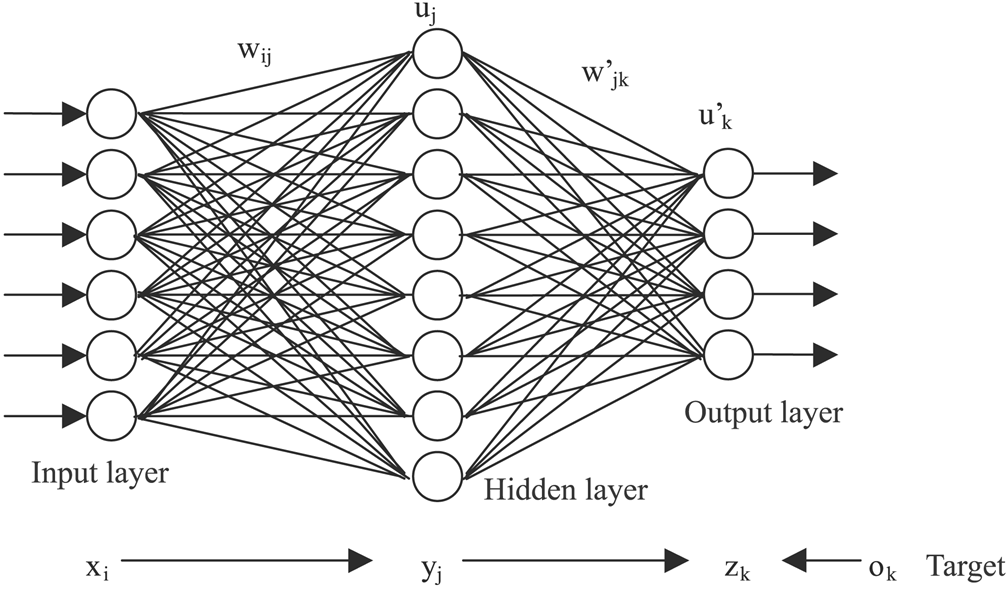
\includegraphics[width=0.7\textwidth]{neuronalesnetzwerk.png}
	\caption{Künstliches Neuronales Netzwerk\protect\cite{annpic}}
	\label{fig:Bild1}
\end{figure}
~\\\\
Jeder Layer besteht aus künstliche Neuronen. Diese haben ihre Namensgebung von aus der Natur stammende Neuron in Gehirnen von Lebewesen. Neuronen sind die Bausteine, aus denen die Gehirne von Lebewesen wie Fischen, Vögeln und Säugetiere zusammen gesetzt sind. Neuronen, oder auch Nervenzellen haben einen Zellkern der Zentrum der Zelle ist. Um sie herum sind Dendriten welche die Verbindung zu anderen Neuronen her stellt. Neuronen sind untereinander mit dem Axonen verbunden, welche an den enden Synapsen haben die Grenze von Axon zur Nervenzelle einen Spalt bilden. Dieser Spalt kann überwunden werden indem von der Synapse Botenstoffe abgesendet werden, die sich dann an den Rezeptor der gegenüberliegenden Synapse anhaften. Diese Übertragung findet statt wenn an der Synapse ein bestimmter Schwellenwert überschritten wurde von elektrischen Reizen, welche die Zelle abfeuert lässt. Künstliche Neuronen haben diesen Schwellenwert durch sogenannte Gewichte w\textsubscript{ij} diese sind auf den Verbindungen zwischen den Neuronen in den unterschiedlichen Layern im KNN (vgl. \ref{fig:Bild2}). Dabei steht i für die Position im Layer und j in welchen Layer sich das Neuron befindet.
\begin{figure}[htbp] 
	\centering
	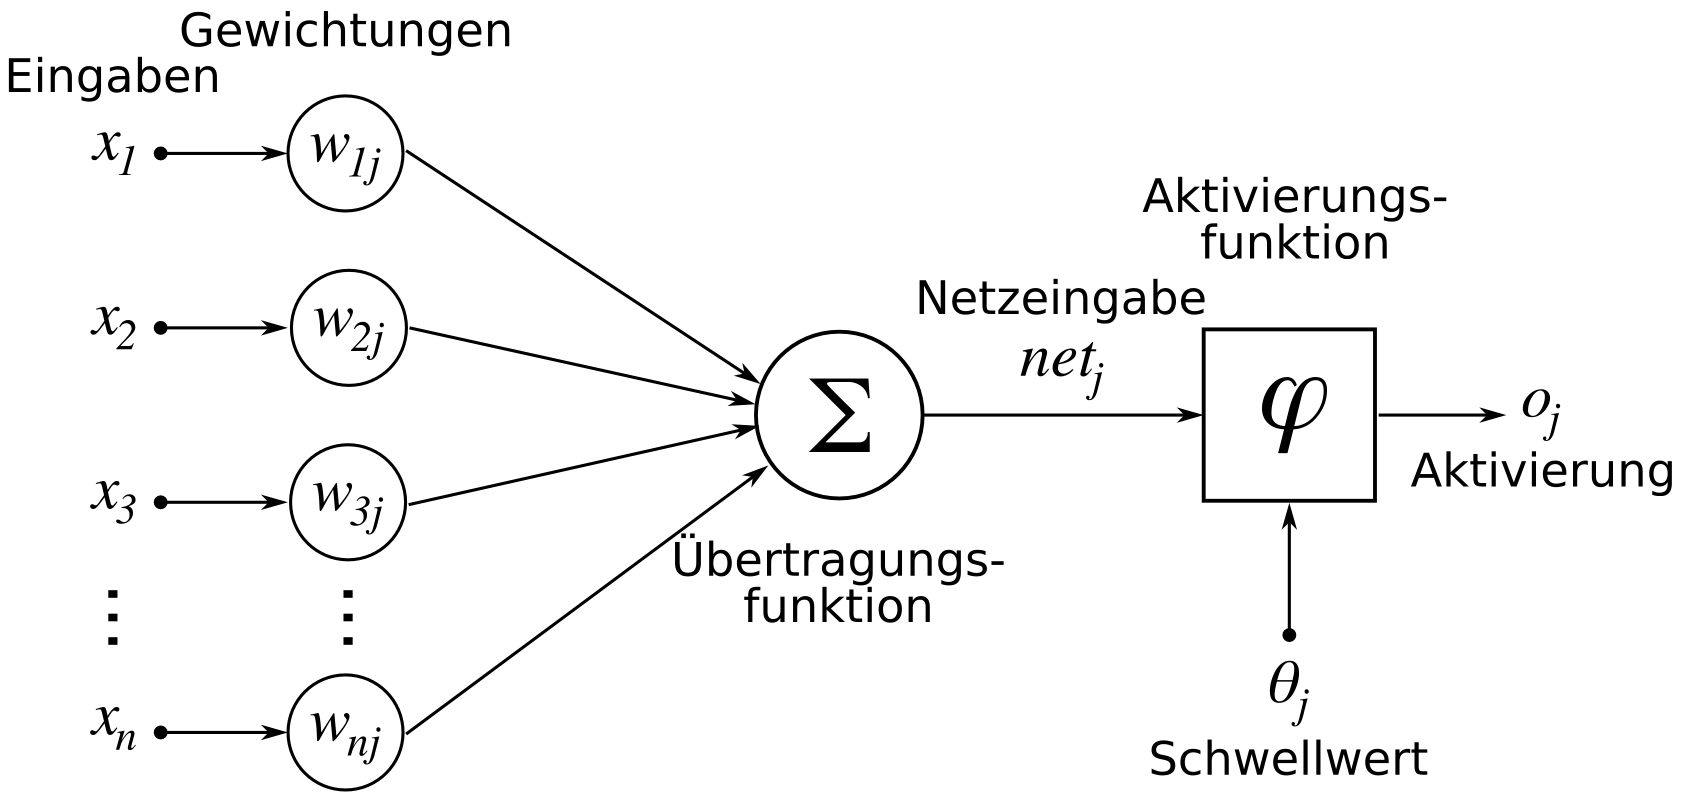
\includegraphics[width=0.7\textwidth]{Neuron.png}
	\caption{künstliches Neuron}
	\label{fig:Bild2}
\end{figure}
Jeder Layer eines KNN besteht aus mehreren Neuronen. Ein Neuron $\theta$ kann mehrere Inputs X\textsubscript{n} erhalten und produziert einen Output $\omega$\. Die Berechnungen, welche von den Neuron durchgeführt werden sind zunächst jeden Input X\textsubscript{n} mit einen Gewicht w\textsubscript{ij} zu multiplizieren. Anschließend wird die Summe von x*w gebildet. Das Ergebnis wird dann in eine Aktivierungsfunktion $\lambda$ gegeben. Ein Neuron ist definiert durch:
\\\\
\begin{math}
y\textsubscript{k} = \lambda(\sum_{j=0}^{m}(w\textsubscript{kj}+x\textsubscript{j})+b\textsubscript{k})                
\end{math}
\\\\
Die Aufgabe der Aktivierungsfunktion $\lambda$  ist es eine nicht lineare Transformation des Inputs zu erzeugen. Damit kann das KNN nicht lineare Funktionen abbilden und somit komplexere Aufgaben lösen. Es gibt unterschiedliche Aktivierungsfunktionen im folgenden werden einige aufgezählt:
\vspace{5 mm}
\begin{description}
	\item[Sigmoid-Funktion]		
	
	\begin{math}
	\sigma(x)=\frac{1}{1+exp(-x)}
	\end{math}
	\vspace{5 mm}
	\item[Softmax-Funktion]
	
	\begin{math}
	\zeta(x)\textsubscript{j} = \frac{e\textsuperscript{x\textsubscript{j}}}{\sum_{k=1}^{K}e\textsuperscript{x\textsubscript{k}}}
	\end{math}
	\vspace{5 mm}
	\item[Rectified Linear Unit (ReLU):]
	
	\begin{math}
	f(x)=\max(0,x) 
	\end{math}
	\vspace{5 mm}
	\item[Leacky Rectified Linear Unit(Leaky Relu):]
	
	\begin{math}
	f(x) = \begin{cases}
	x  	 & \quad \text{if } x > 0\\
	0.01x & \quad \text{sonst} 
	\end{cases}
	\end{math}
	\vspace{5 mm}
\end{description}
\vspace{5 mm}
Der Funktionsplot von Sigmoid Funktion kann Abb.\ref{fig:Bild3} entnommen werden. Dieser veranschaulichen den Wertebereich, welcher von den Aktivierungsfunktion angenommen werden kann und ihren Verlauf. 
\begin{figure}[htbp] 
	\centering
	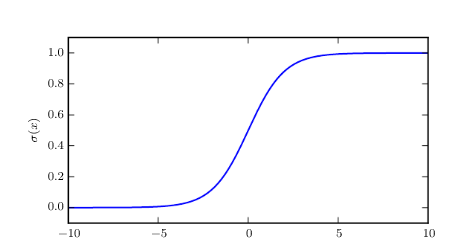
\includegraphics[width=0.5\textwidth]{sigmoid.png}
	\caption{Sigmoid Funktion}
	\label{fig:Bild3}
\end{figure}

\newpage
\subsubsection{Ziel-Funktion}\label{sec:Zielfunktion}
~\\\\
Die Ziel-Funktion oder auch Loss-Funktion genannt J($\theta$), muss differenzierbar sein wobei $\theta$ das KNN ist und J für die Zielfunktion steht. Das heißt die Funktion f: D $\to$ R ist differenzierbar an der Stelle x\textsubscript{0}. Wenn nun $f^\prime$: x $\to$ f(x) an jedem Punkt x\textsuperscript{n} ableitbar ist, ist f differenzierbar. Die Aufgabe der Ziel-Funktion ist es zu messen wie gut unsere Model $\theta$ f*(x) approximiert. Es wird der Begriff Kosten verwendet, wie viel Kosten erzeugt das Model beim Lösen der zugewiesenen Aufgabe. Die Wahl, welche Ziel-Funktion gewählt wird ergibt sich aus der Aufgabe des KNN. Diese kann beispielsweise für Klassifikations oder Regressions Aufgaben hergenommen werden. Bei Regression soll eine kontinuierliche Variable von $\theta$ als Output generiert werden, wohingegen bei Klassifikationsproblemen der Output Klassen-Labels darstellt\cite{Grundlagen}. Es gibt verschiedene Ziel Funktionen im folgenden wird die Cross Entropy Loss Function vorgestellt \cite{crossentropy}. Diese kann verwendet werden um beispielsweiße Klassikationsprobleme zu lösen. Diese ist definiert als:
\\\\
\begin{math}
\hat{q}(c\mid x)=\displaystyle\arg\min_{q(c\mid  x)}\{-\displaystyle\sum_{n}{\log q(c\textsubscript{n}\mid x\textsubscript{n})}\}
\end{math}
\\\\
Wobei  x\textsubscript{n}:n=1,...,N die Trainingsdaten sind und c\textsubscript{n}:n=1,...,N die möglichen Klassen. Der Output ist die Wahrscheinlichkeit zwischen 0 und 1, ob  x\textsubscript{i} $\in$ der bestimmten Klasse enthalten ist. Auch kann sie hergenommen um zu messen wie hoch die Differenz zwischen zwei Wahrscheinlichkeitsverteilungen ist.


\subsubsection{Backpropagation Algorithmus}\label{sec:test}
~\\\\
Um nun KNNs zu trainieren und den gewünschten Output y zu generieren wird der Backpropagation Algorithmus benutzt. Dieser zählt zu den Optimierungs Algorithmen für KNN und arbeitet schneller und effizienter auf Neuronalen Netzwerken als andere Optimierungsalgorithmen vor ihm. Das mathematische zugrundeliegende Konzept ist ein Optimierungsproblem der die partitielle Ableitung von  $\frac{\partial J}{\partial w}$, wobei J die Zielfunktion und w die Gewichte im zu optimierenden Neuronalen Netzwerk, sind. Für eine Funktion $f$(x) = y ist die Ableitung definiert als $f^\prime$(x) oder $\frac{dy}{dx}$ und gibt die Steigung der Funktion an Punkt x an. Durch die Steigung am Punkt x ist man nun in der Lage eine Änderung von der Ableitung x dahin gehend  zu optimieren \cite{Grundlagen}. Dieses Verfahren hilft dabei das KNN  dahingehen zu optimieren den gewünschten Output y zu erlangen. Dieses Ziel wird durch die Ziel-Funktion einen KNN beschrieben(vgl. \ref{sec:Zielfunktion}). Das Verfahren wird in Abb. \ref{fig:Bild4} veranschaulicht.   
\\
\begin{figure}[htbp] 
	\centering
	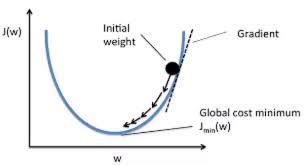
\includegraphics[width=0.5\textwidth]{gradient.png}
	\caption{Optimierung einer Zielfunktion}
	\label{fig:Bild4}
\end{figure}
\\
Wenn nun $f^\prime$(x) = 0 gibt es keinerlei Information über die Steigung. Dies ist aber kein Indiz dafür,dass $f$ ein Optimum erreicht hat. Es könnte, wie in Abb. \ref{fig:Bild5} unten dargestellt ein lokales Minimum sein, was bedeutet, dass an diesen Punkt ein Minimum erreicht ist aber im Funktionsverlauf ein noch niedrigeres Minimum vorhanden ist. Oder einen Sattelpunkt welche einen Übergang zu einen anstieg der Funktion bildet.
Ist nun die die Funktion $f$ definiert als $f$: $\mathbb{R}$\textsuperscript{n} $\rightarrow$  $\mathbb{R}$ hat sie als Input mehrere Variablen. Die partielle Ableitung $\frac{\partial f(x)}{\partial x\textsubscript{i}}$ zeigt an wie sehr sich $f(x)$ ändert wenn x\textsubscript{i} geändert wird. Der Gradient $\nabla\textsubscript{x}f(x)$ ist ein Vektor, welcher alle partiellen Ableitungen von $f$ enthält. Nun kann f optimieren  werden, in dem, in die Richtung die Gewichte w\textsubscript{ij} von $\theta$ dahin gehen verändert werden in dem das Gradientenverfahren absteigend zu $f^\prime$(x) = 0 optimiert wird. Dieses Verfahren wird Gradient Descent genannt \cite{Grundlagen}. Beim Mini-batch Gradient Descent wird die Anpassung der Gewichte während des Trainings in n Batches unterteilt. Die Batches bestehen aus jeweils i Datensätze welche aus dem Trainingsdatensatz enthalten sind. Nach dem der Gradient für die i Datensätze des jeweiligen Batch berechnet wurden, werden die Gewichte $\theta$ des ANN angepasst und der nächste Batch wird zum trainieren verwendet. Solange bis e Epochen wobei e die Durchläufe des kompletten Trainingdatensatzes stehen, passiert sind. Dieses Verfahren führt zu stabileren Trainingsergebnisse \cite{batchgradeint}.

\begin{figure}[htbp] 
	\centering
	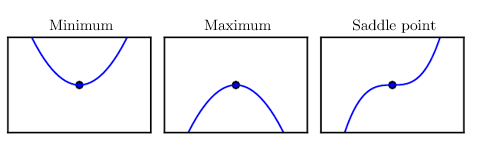
\includegraphics[width=1.0\textwidth]{saddle.png}
	\caption{Minimum,Maximum und Sattelpunkt einer Zielfunktion\protect\cite{saddleimage}}
	\label{fig:Bild5}
\end{figure}


\subsubsection{Momentum}\label{sec:momentum}
~\\\\
Momentum hat das Ziel das Gradientenverfahren des Backpropagation Algorithmus \ref{sec:test} zu beschleunigen, um ein effizienter Ergebnis herbei zu führen und ein schnelleres Lernen erreichen. Definiert ist dies durch:
\\\\
\begin{math}
v\textsubscript{t+1} =\mu v\textsubscript{t}-\epsilon\nabla$f$(\theta\textsubscript{t})
\theta\textsubscript{t+1}= \theta\textsubscript{t}+v\textsubscript{t+1}
\end{math}
\\\\
wobei $\epsilon$ $>$ 0 die Lernrate ist,  $\mu$ $\in$ [0,1] das Momentum und $\nabla$f($\theta\textsubscript{t}$) der Gradient von $\theta\textsubscript{t}$ ist. Je größter das Momentum, desto schneller bewegt sich der Gradient abwärts. Da dieser am Anfang einer Lernphase der üblicherweise hoch ist empfiehlt sich zunächst mit einen niedrigen Momentum zu Arbeiten da sonnst die Gefahr besteht über das globale Optimum hinaus zuschießen. Wenn nun das Training stagniert, was aus Gründe der Aufbau der Zielfunktion zurückzuführen ist das zur nähe des globalen Optimums flache Täler entstehen welche das Trainings verlangsamen und es zu keiner Verbesserung kommt, kann man durch Momentum erzwingen größere Gradienten Sprünge einzugehen. Und sich somit schneller zu einen globalen Optimum zu bewegen oder aber aus einen lokalen Optimum hinaus Richtung eines globalen Optimum zu bewegen kann Momentum benutzt werden\cite{momentum}.

\subsubsection{Regularization}
~\\\\
Ein Problem welches alle Machine Learning Anwendungen teilen ist es wenn der Trainingsalgorithmus zunächst eine gutes Trainingsergebnis erzielt, aber dann auf dem Testdatensatz ein schlechtes Ergebnis erlangt, was Overfitting genannt wird. Es gibt einige Möglichkeiten die eingesetzt werden können, welche dann aber ebenfalls auch das Trainingsergebnis verschlechtern. Man spricht davon das Model zu Regularizieren.

\begin{description}
\item[Data Argumentation]
~\\\\
Je mehr Daten beim Training verwendet werden desto mehr kann generalisiert werden. Data Argumentation heißt, dass man mehr Datensätze erstellt. Dies kann durch eine Veränderung der Trainingsdatensätze im Allgemein geschehen \cite{Grundlagen}, wenn man beispielsweise 3D-Punktwolken rotiert, um diese mehrfach zu nutzen. Eine weitere Möglichkeit ist es, bestimmte Datenpunkte in einen Datensatz ändern indem man ein Objekt, welches auf einem Bild dargestellt wird, verkleinert oder vergrößert\cite{Grundlagen}. \\
\item[Dropout]
~\\\\
Bei Dropout wird während des Lernprozess ein gewisser Prozentsatz der Neuronen in jedem Layer nicht verwendet. Dies zwingt das Netzwerk, welches sonnst die Abhängigkeiten zwischen den Neuronen lernt, eine generalisiertere Lösung zu finden\cite{dropout}.\\
\item[L2-Regularization]
~\\\\
Dabei wird das Gewicht des Neurons während des Trainings näher zu seinem Ursprung, dass heißt dem Wert seiner Initialisierung, gedrängt. Dies passiert indem ein Regularisierungswert $\Omega$ = $\frac{1}{2}||w||\frac{1}{2}$ an die Zielfunktion gehängt wird. Dieses sorgt dafür, dass während dem Training der Gewichts Vektor welche durch das Gradienten Verfahren ermittelt wird, schrumpft, was für eine höhere Varianz während des Trainings sorgt, welches wiederum das KNN dazu zwingt mehr zu generalisieren\cite{Grundlagen}.\\ 
\end{description}

\subsubsection{Batch Normalisation}
~\\\\
Wie in Kapitel \ref{sec:test} gezeigt hat das stochastischen Gradienten Verfahren Vorteile gegenüber dem normalen Gradienten Ermittlung Verfahren beim Training von KNN. Dadurch das der Input in jeden Layer abhängig von den vorherigen Layern ist können Änderungen von Werten in frühen Layern des KNN große Auswirkungen in tieferen Layern im Netzwerk haben.
Dadurch resultiert dass in Trainingsabläufen die Verteilung der Gewichte in den jeweiligen Layern verlangsamt wird. Batchnormalization soll die Werteänderung von Gewichten verringen. Dieses Problem wird auch Covariance Shift genannt. Um dies zu verhindert zeigten Sergey Ioffe und Christian Szegedy \cite{batchnorm} eine Methode, welche Batch Normalisation genannt wird. Je mehr Layer das Netzwerk hat desto stärker ist der Covariance Shift. Batch Normalisation besteht aus zwei Algorithmen. Algortithmus 1 verändert den eigentlichen Input von Layer n zu einen normalisierten Input y und Algorithmus 2 verändert das eigentliche Training eines Batch normalisierten Netzwerkes\cite{batchnorm}.
\\\\
\begin{algorithm}[H]
	Input: Werte von x über einen Mini-Batch $B$ = \{$x\textsubscript{1},...,x\textsubscript{n}$\}\\
	\begin{math}
	\mu\textsubscript{$B$}\leftarrow\frac{1}{m}\displaystyle\sum_{i=1}^{m}$x$\textsuperscript{i}
	\end{math}\\
	\begin{math}
	\sigma\textsubscript{$B$}\leftarrow\frac{1}{m}\displaystyle\sum_{i=1}^{m}($x$\textsuperscript{i} - \mu\textsubscript{$B$})\textsuperscript{2}
	\end{math}\\
	\begin{math}
	\hat{x\textsubscript{i}}\textsubscript{$B$}\leftarrow\frac{x\textsubscript{i}-\mu\textsubscript{$B$}}{\sqrt{\sigma\textsubscript{$B$} + \epsilon}}
	\end{math}\\
	\begin{math}
	$y$\textsubscript{i}\leftarrow\gamma\hat{x\textsubscript{i}} + \beta \equiv BN\textsubscript{$\gamma$;$\beta$}($x$\textsubscript{i})
	\end{math}\\
	Output: \{$y$\textsubscript{i}=BN\textsubscript{$\gamma$;$\beta$}($x$\textsubscript{i})\}
	\caption{Batch Normalisierung angewand auf x über Input bei Mini-Batch  }	
\end{algorithm}
~\\\\
In Schritt 2 des Algorithmus 1 wird der Erwartungswert für alle Inputs von Mini-Batch B berechnet und in Schritt 3 die Varianz. In Schritt 3 wird nun der der normalisierte x\textsubscript{i} berechnet welche dann mit $\beta$ und $\gamma$ multipliziert werden. Diese Werte sind neue Gewichte im Neurnonalen Netzwerk welche während des Trainingsprozesses angepasst werden. $\epsilon$ in der Gleichung in Zeile 4 ist nur dafür da damit nicht durch 0 geteilt werden kann. In Zeile 8 - 11 werden die Inferenz Schritte beschrieben, bei welchen der Minibatch des Trainings ersetzt wird \cite{batchnorm}. In Abb. \ref{fig:Bild6} ist veranschauchlicht wie die Batch-Normalization-Layer in das KNN eingebaut werden. 

\begin{figure}[htbp] 
	\centering
	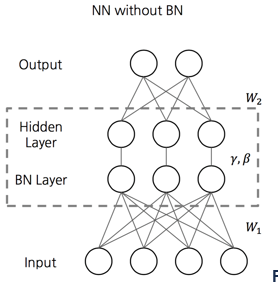
\includegraphics[width=0.5\textwidth]{batchnorm.png}
	\caption{Neuronales Netzwerk mit Batch-Normalization-Layer\protect\cite{batchnormweb}}
	\label{fig:Bild6}
\end{figure}

\subsection{Datenformat Punktwolken}\label{sec:punktwolken}

Punktwolken sind eine Menge von N Punkten, welche im Vektorraum dargestellt werden können. Jeder Punkt n $\in$ N wird durch seine (x,y,z) Koordinaten im Euklidischen Raum dargestellt. Punkte können zusätzliche Features gegeben werden, wie Farbe oder Material. Es gibt unterschiedliche Dateiformate, welche für die Abspeicherung von Punktwolken herangezogen werden können bespiele dafür sind PLY, STL oder OBJ. Das Polygon File Format(PLY) speichert die einzelnen Koordinaten in einer Liste, welche Vertex List genannt in. In Abb. \ref{fig:Bild7} kann eine Beispieldatei entnommen werden in der dieser Aufbau dargestellt ist. 
\\
\begin{figure}[htbp] 
	\centering
	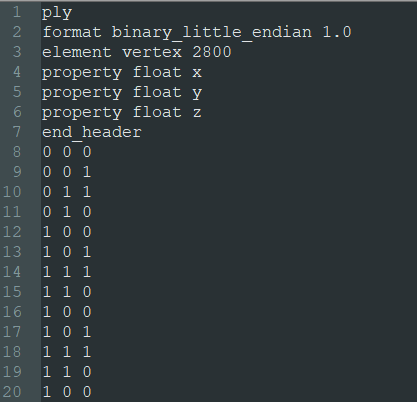
\includegraphics[width=0.4\textwidth]{plyexample.png}
	\caption{Polygon File Format}
	\label{fig:Bild7}
\end{figure}
\\
Punktwolken können als Menge betrachtet werden. Die jeweiligen Punkte sind geordnet in dieser Listen gespeichert jedoch spielt es keine Rolle für den Punktwolkencompiler bei der Visualisierung der Liste an welcher Listenposition ein jeweiliger Punkt geführt wird, die Liste wird jedes mal gleich angezeigt, egal welche Permutation der einzelnen Punkte in der Liste durchgeführt wird. In Abb. \ref{fig:Bild8} kann eine visualisierte Punktwolke eines Tabakblattes entnommen werden. 
\\
\begin{figure}[htbp] 
	\centering
	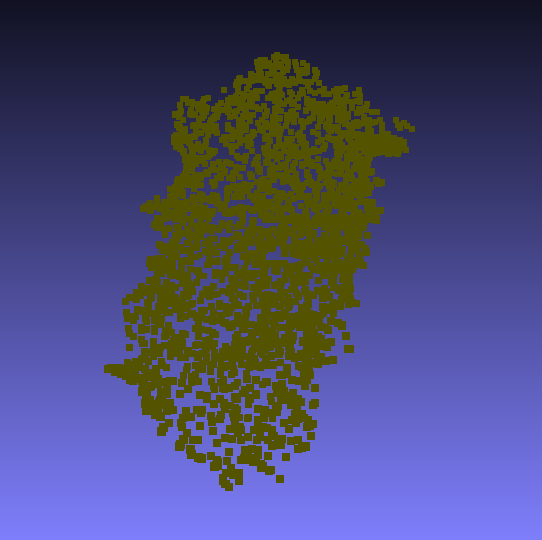
\includegraphics[width=0.5\textwidth]{leaf1.png}
	\caption{Visualisierte Punktwolke eines Tabakblattes}
	\label{fig:Bild8}
\end{figure}
\newpage
\subsubsection{Datenaufnahme von Tabakpflanzen}
~\\\\
Die Punktwolken können Beispielsweise von den TERRA-REF Feld Scanner von der University von Arizona Maricopa Agricultural Center and USD Arid Land Researh Station in Maricopa aufgenommen werden. In Abb. \ref{fig:Bild9} ist  Recht eine Skizze dargestellt. In Abb. \ref{fig:Bild9} Links ist der Scankopf des TERRA-REF dar gestellt.
\begin{figure}[htbp] 
	\centering
	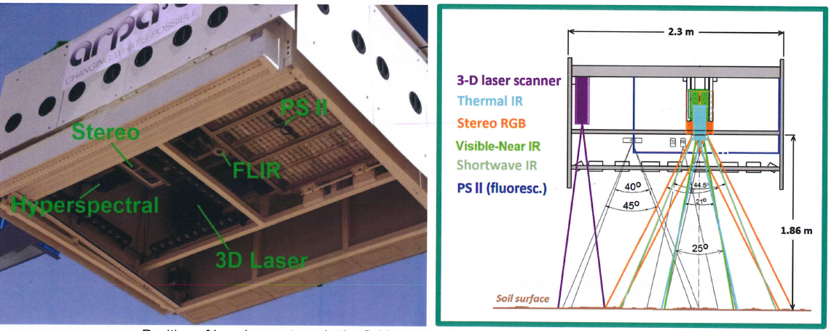
\includegraphics[width=0.5\textwidth]{lematech_2.png}
	\caption{Scankopf und Scanaufbau für die 3D-Punktwolken Gewinnung}
	\label{fig:Bild9}
\end{figure}
Der 3D Laser Scanner erzeugt 3D Punktwolken. Dabei werden die Objekte durch den Scanner erfasst und eine 3D Repräsentation, welche durch Punkte in einen 3 Dimensionalen Koordinaten System erfasst werden können, dargestellt. Dabei wird ein Laser über das zu scannende Objekt gefahren durch reflektion des Laserstrahls auf der Oberfläche des Objektes können x,y,z Koordinaten des jeweiligen Punktes auf den Objekt bestimmt werden. Eine 3D-Scan einer Tabakpflanze kann in Abb.\ref{fig:Bild100} entnommen werden. Diese wurden in dieser Arbeit von Fraunhofer-Institut für Integrierte Schaltungen zur Verfügung gestellt. Da nun beim Scannen eines Objektes durch andere Objekte die Oberfläche verdeckt sein können. Wie beispielsweise beim Scannen von Tabakpflanzen, Blätter den Scankopf es nicht Möglich macht Objekte unterhalb dieses zu erreichen. Können Scans unvollständig sein. Dieses Problem für zu den Ziel dieser Arbeit, eine Möglichkeit zu Prüfen diese unvollständigen Punktwolken zu vervollständigen. Genaueres zum diesen Thema in Kapitel \ref{sec:rekdaten}. 
\begin{figure}[htbp] 
	\centering
	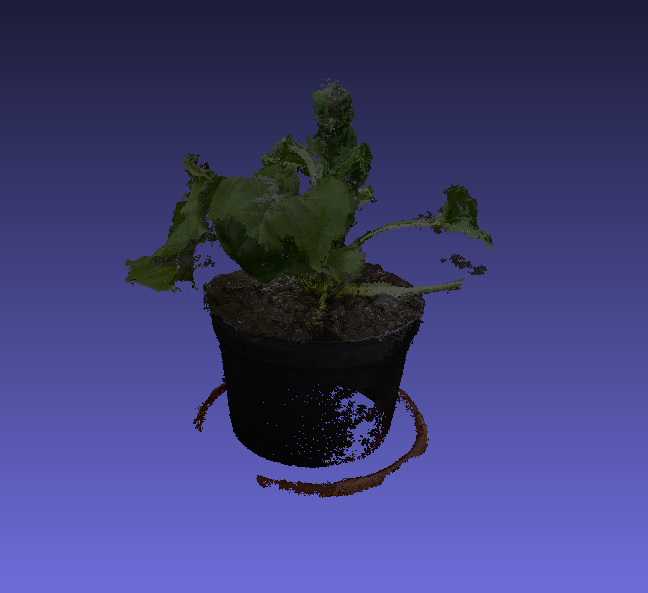
\includegraphics[width=1.0\textwidth]{plant.png}
	\caption{3D Punktwolke einer Tabakpflanze}
	\label{fig:Bild100}
\end{figure}
\newpage
\subsubsection{Die Schwierigkeit bei mit 3D-Data bei Machine Learning Ansätzen}\label{sec:3dprobleme}
~\\\\
Vergleicht man 3D-Data auf ihre Dimensionalität mit anderen Datenformaten wie Bild,- Audio-, und Textdateien steigt der Informationsgehalt und dadurch auch die Komplexität für das Anwenden von Maschine Learning Algorithmen enorm. Besonders bei Nicht-Euklidischen 3D-Daten wie Punktwolken, welchen keine Struktur zu Grunde liegt ist dieses gegeben \cite{3dprob}.
\\\\
Wie im Kapitel \ref{sec:punktwolken} gezeigt, sind Punktwolken als Menge gespeichert, in der keine Relation untereinander besteht. Was bedeutet, dass es für den Punktwolkencompiler nicht von Relevanz ist auf welchem Platz die einzelnen Punkte abgespeichert werden. Die Punktwolke wird immer gleich angezeigt, egal in welcher Permutation der einzelnen Punkte abgespeichert abgespeichert werden. Vergleicht man nun ein Bild mit 512 Pixeln und 3 RGB-Farbkanälen ist einer Dimension von 391680 erreicht. Vergleicht man dies mit einer Punktwolke in einen 125 cm \textsuperscript{3}großen Bereich. Da die einzelen Koordianten eines Punktes als Rationale Zahlen dargestellt werden und rationale Zahlen abzählbar unendlich sind ist der Suchraum unendlich groß. Dies führt zu einen erheblichen mehr Aufwand für Machine Learning Ansätzen wie, Deep Learning für Punktwolken.
\\\\
Ein weitere Schwierigkeit, die für Deep Learning mit Punktwolken besteht ist, dass die aus Kapitel Convolutional Neural Network beschrieben Convolutionel-Layer einen großen Beitrag bei dem Fortschritt von Deep Learning gebracht hat. Da sie helfen die Strukturen von strukturierten Daten zu lernen und den latenten Raum zu entdecken. Da jedoch Pointclouds unstrukturiert sind hilft es nicht unbedingt diese Tools auch bei Punktwolken einzusetzen\cite{3dgan}.  

\subsection{Convolution Neural Networks}

Convolution Neural Netzworks(CNN) sind eine besondere Art von künstlichen neuronalen Netzwerken, sie sind dafür konzipiert auf Datensätzen zu arbeiten welche in eine Matrix Form gebracht worden sind. Der Input eines CNN können beispielsweise Bilder sein welche durch die Matrix A =
$
\begin{bmatrix}
a_1	& a_1	& \dots	 & a_n     \\
b_1	& b_2 	& \dots  & b_n	  \\
\vdots	& n_n 	& \ddots & \vdots \\
x_1 	& x_2 & x_3	 & x_n
\end{bmatrix}
$
\\\\dargestellt werden. Jedes Element x\textsubscript{ij} stellt einen Pixel eines Bildes da, wobei x\textsubscript{n} $\in$ [0,255] . Die Matrix A\textsuperscript{w$\cdot$b$\cdot$c} stellt w$\cdot$b$\cdot$c = N dimensionale Matrix da. Wobei w die Länge und b Breite des Bildes entspricht. c sind die Farbspektren eines Bildes und sind in einen RGB-Farbraum 3 beziehungsweiße in einen schwarz-weiß Bild 1. Nachdem  der Input eines CNN definiert ist kommt nun der Aufbau. CNN setzen sich aus mehrere Schichten von Convolution Layern zusammen. Ein Netzwerk kann mehrere N-Layer haben. Wobei jeder Layer aus mehreren Convolution oder auch Kernels genannt, zusammengesetzt ist. Ein Aufbau kann aus Abb. \ref{fig:Bild10} entnommen werden\cite{Grundlagen}.
\begin{figure}[htbp] 
	\centering
	\includegraphics[width=1.0\textwidth]{convol.png}
	\caption{Convolutional Neural Network}
	\label{fig:Bild10}
\end{figure}
Die Kernels, also die einzelnen Filter, von denen jeder N-Layer k besitzt sind K\textsuperscript{n$\cdot$n} Matrizen jedes k\textsubscript{ij} in einem Filter einspricht einen, aus den üblichen Neuronalen Netzwerk Architektur bekannten Gewichte. Diese Gewichte werden dann durch den Backprobagation-Algorithmus in der Trainingsphase des Netzwerkes angepasst um den Verlust der Ziel-Funktion durch bestimmten des Gradianten zu minimieren. Das in Abb. \ref{fig:Bild10} dargestellte Subsampling ist der Output aus den Convolutional Layern\cite{Grundlagen}. 
\\\\
Da Input und Kernel unterschiedliche Größen haben und man den gesamten Input mit den Kernel abdecken möchte, bewegt sich der Filter um s Position auf den Input und führt erneut einen Berechnungschritt durch. Dieser Vorgang wird Stride genannt. An jeder Position wird das Produkt von jeden x\textsubscript{ij} des Input und k\textsubscript{ij} des Kernel durchgeführt.  Anschließend werden alle Produkte aufsummiert. In Abb. \ref{fig:Bild11} ist dieser Vorgang verdeutlicht. Zusätzlich gibt es die Möglichkeit für das sogenannte Zero Padding P. Dabei werden mehrere 0 um die Input Feature Map, am Anfang und Ende der Axen anfügt. Dies ist notwendig wenn Kernel und Input Größe nicht kompatible zueinander sind. Die Anzahl der möglichen Positionen ergeben sich aus der Kernel Größe und den Input des jeweiligen Kernel sowie des Strides. Die Output Größ W kann berechnet werden durch W = (W-F+2P)/s+1 berechnet werden. Wobei F für die Größe des Kernel steht \cite{conv}.
\newpage
\begin{figure}
	\centering
	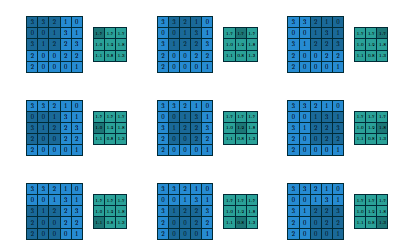
\includegraphics[width=0.8\textwidth]{conv.png}
	\caption{Convolution Beispiel\protect\cite{conv}}
	\label{fig:Bild11}
\end{figure}
Um  besser zu verstehen welche Auswirkungen die Anzahl der Kernels in Layer n auf die Größe des Outputs von n und die Anzahl der Kernels in Layer n+1 für den nächsten Layer haben, wird ein Beispiel aufgezeigt. Der erste Layer hat 20 Kernels mit der Größe 7x7 und Stride 1. Der Input A für einen Kernel K ist ein 28x28 Matrix. Der Output aus diesen Filter sind 20 22x22 Feature Maps. Wäre der Input ein 28x28x3 Bild mit 3 RGB Channels sein, der Output 60 22x22 Feature Maps. Allgemein kann Convolution Layer als Supsampling gesehen werden und Stride gibt an wieviele Dimensionen bei diesen Prozess pro Convolution Layer entfernt werden soll. Der letzte Layer ist ein Fully-Connected Layer welcher den typischen Anforderungen von ANN entspricht \cite{conv}.  
\\\\
Transposed Convolution, auch genannt Fractionally Strided Convolution oder Deconvolution, ist eine Umkehrfunktion von der üblichen Convolution. Es verwendet die gleichen Variablen wie Convolution. Dabei wird ein Kernel K mit der Größe N x N definiert der Input I mit der Größe N x N und Stride s = 1. Deconvolution kann wie Convolution angesehen werden mit  Zero Padding auf dem Input.  Das in Abb. \ref{fig:Bild12} gezeigte Beispiel zeigt einen deconvolution Vorgang mit eine 3x3 Kernel über einen 4x4 Input. Dies ist gleich mit einen Convolution Schritt mit einen 3x3 kernel auf einen 2x2 Input und einer 2x2 Zero Padding Grenze. Convolution ist Supsampling und mit Deconvolution wird Upsampling betrieben. Durch diesen Schritt kommt es zu einer Dimensionserhöhung des Inputs. Die Gewichte der Kernels bestimmen wie der Input transfomiert wird. Durch mehrere Schichten von Deconvolution Layer kann von einer Input Größe NxN auf eine Output Größe KxK, wobei K $>$ N mit Abhängigkeit von Kernel und Stride abgebildet werden\cite{conv}. 

\begin{figure}[htbp] 
	\centering
	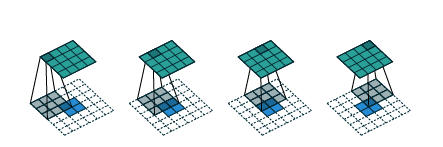
\includegraphics[width=1.0\textwidth]{decon.png}
	\caption{Deconvolution Beispiel \protect\cite{conv}}
	\label{fig:Bild12}
\end{figure}
\newpage
\subsection{Autoencoder}\label{sec:autoencoder}

Autoencoder gehören zu den generativen Modellen im Bereich des Machine Learnings. Generative Modelle haben das Ziel eine Wahrscheinlichkeitsverteilungen zu erlernen. Anschließend kann diese als ein Modell genutzt werden um Samples aus dieser zu erzeugen. Die Modelle können dabei beispielsweise auf KNN oder Markov Chains trainiert werden. Im folgenden liegt der Fokus auf KNNs. Allgemein gehalten können jegliche Typen von Daten wie Text, Bild oder Audiodateien für generative Modelle herangezogen werden. Es gibt unterschiedliche Typen von generativen Modellen, welche sich vom Aufbau des Neuronalen Netzwerk und der Zielfunktion unterscheiden. Beispiele dafür sind Boltzmann Maschine, Autoencoder oder Deep Belief Networks\cite{Grundlagen}. 
\\\\
Autoencoder sind eine andere Art von Model aus den Bereich der generativen Modelle. Ihre Aufgabe besteht darin einen Input zu komprimieren und aus der komprimierten Information den Input wieder herzustellen. Die Technik auf welche Autoencoder zurückgreifen, nennt sich Dimensionreduktion. Dabei wird die Dimension der Daten so reduziert um Informationen bei zu behalten, welche als relevant gelten. Diese Technik findet auch in anderen Machine Learning Anwendung, wie beispielsweise der Principale component anaysis(PCA) Anwendung\cite{dimreduction}.  Ein Autoencoder besteht aus 2 Bestandteilen. Erstens einen Encoder e dargestellt als z=$f$(x) welcher einen Input x $\in$ von $x\textsuperscript{i}$ wo x ein Vektor der Länge i ist und damit die Input Dimension bestimmt. Dieser wird durch den Encoder auf einen Vektor $z\textsuperscript{k}$ abgebildet wobei k$<$i ist. Zweitens der Decoder d dargestellt als x`=g(z), bekommt als Input $z\textsuperscript{k}$ und bildet z auf $r\textsuperscript{l}$ ab wobei l = i. Und somit die gleiche Dimension wie der Input. Aufgabe ist es nun, dass der Encoder den Input x so gut komprimiert, dass der Decoder es schafft das x $\thickapprox$ x`. Eine grafische Darstellung kann aus Abb. $\ref{fig:Bild13}$ entnommen werden\cite{Grundlagen}. 
\\\\
Der Autoencoder wird durch den in Kapitel \ref{sec:test} vorgestellten Algorithmus trainiert und erlernt so können beispielsweise durch Fully-Connected-Layer,  Convo-lutional-Layer oder Deconvolutional-Layer modelliert werden. Eine Metrik um zu messen wie das Model seine Aufgabe erfüllt, könnte beispielsweiße die Cross-Entropy-Funktionen sein welche schon in Kapitel \ref{sec:Zielfunktion} vorgestellt worden ist. Weitere spezifische Zielfunktionen für Autoencoder welche mit 3D Punktwolken arbeiten und für die folgende Arbeit von belangen sind, werden nun vorgestellt.
\begin{figure}[htbp] 
	\centering
	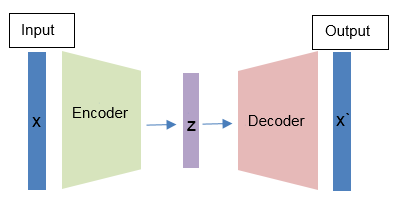
\includegraphics[width=1.0\textwidth]{autoencoder2.png}
	\caption{Autoencoder}
	\label{fig:Bild13}
\end{figure}
~\\\\
Bei Punktwolken als Datentyp erzielt die Cross-Entropy-Funktion keine guten Ergebnisse da diese invariant zu ihrer Permutation sind. Da dieser Arbeit der Input 3d Pointcloud sind und diese Sets  invariant zu ihren Permutationen sind. Ändert sich Anordnung meiner einzelnen Punkte in mein Set bleibt das dargestellte Ergebnis unverändert.  Deshalb kann nicht auf übliche Zielfunktionen welche für strukturierte Daten wie Bilder verwendet werden, zurück gegriffen. Die Herausforderung besteht darin zwischen zwei unterschiedliche Sets von Punkten heraus zu finden, wie hoch die Diskrepanz zwischen den beiden Sets ist\cite{invariant}. 
\\\\
Eine Möglichkeit, speziell für Autoencoder, welche mit Punktwolken arbeiten, ist die Earth Mover Distance(EMD). Bei dieser sind X\textsubscript{1} und X\textsubscript{2} zwei Punktwolken mit jeweils x\textsubscript{n} definierten Punkten\cite{autoencoderloss}. Definiert ist sie durch die Funktion:
\\\\
\begin{math}
d\textsubscript{EMD}=\min_{\theta : X\textsubscript{1}\rightarrow X\textsubscript{2}}  \sum_{x\in X\textsubscript{1}}|| x - \theta(x)||\textsubscript{2};wobei\;\theta: X\textsubscript{1} \rightarrow X\textsubscript{2}\, bijektiv\, ist 
\end{math}
\\\\
Grafisch kann man sich die Berechnung wie in Abb. \ref{fig:Bild14} darstellen. Ein Punkt von x\textsubscript{n} $\in$ X\textsubscript{1} wird den nähsten Punkt y\textsubscript{n} $\in$  X\textsubscript{2} zugewiesen. Wobei die Distanz durch die Euklidische Distanz der jeweiligen Punkte ermittelt wird. 
\begin{figure}[htbp] 
	\centering
	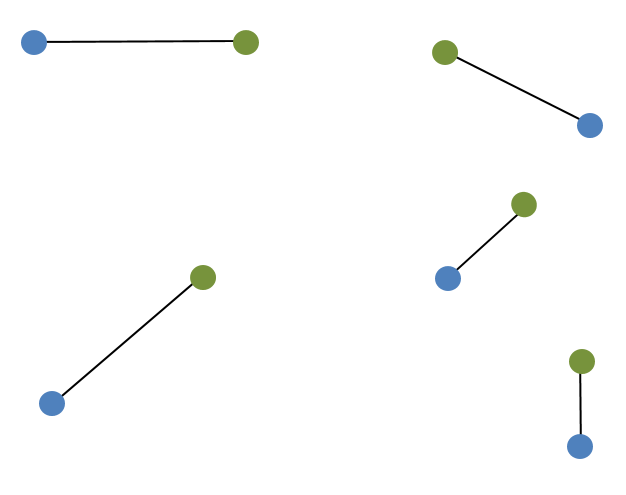
\includegraphics[width=0.5\textwidth]{emd_distance.png}
	\caption{Earth Mover Distance}
	\label{fig:Bild14}
\end{figure}		
Eine weitere Möglichkeit ist die Chamfer Distance(CD). Wie auch zuvor sind  X\textsubscript{1} und X\textsubscript{2} zwei Punktwolken mit jeweils x\textsubscript{n} definierten Punkten\cite{autoencoderloss}. Definiert ist sie durch die Funktion:
\\\\
\begin{math}
d\textsubscript{CD}(X\textsubscript{1},X\textsubscript{2})=\sum_{x\in X\textsubscript{1}} \min_{y \in X\textsubscript{2}}||x-y|| + \sum_{y\in X\textsubscript{2}} \min_{x \in X\textsubscript{2}}||x-y||
\end{math}
\\\\
Der Unterschied ergibt sich zwischen den beiden Metriken, dass bei der EMD von der Ausgangswolke die Punkte zu der anderen jeweils optimiert werden. Wohingegen bei der CD die Distanzen von und zu der Ausgangspunktwolke berechnet werden. Dies geht aus den Abb. \ref{fig:Bild15} hinaus in welche die Distanzberechnung der einzelnen Punkte dargestellt wird\cite{autoencoderloss}.

\begin{figure}[htbp] 
	\centering
	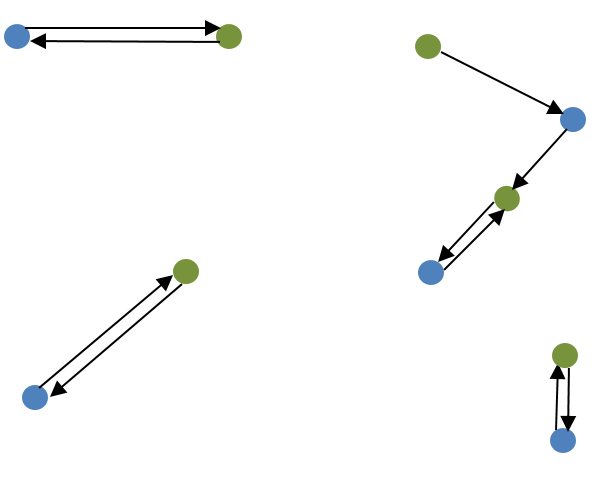
\includegraphics[width=0.5\textwidth]{champfer.png}
	\caption{Chamfer Distance}
	\label{fig:Bild15}
\end{figure} 
\newpage
\subsection{Generative Adversarial Network}
GAN arbeiten nach dem Maximum Likelihood Schätzverfahren (ML-Schätzer) in dem die Parameter $\theta$ dahingegen angepasst werden, dass die unsere beobachtetet Daten am ehesten passen. Man kann ML-Schätzer als Kulback-Leibler(KL) Divergenz darstellen und das generative Modelle das Ziel haben die KL Divergenz zwischen den Trainingsdaten P\textsubscript{r} und den generierten Daten P\textsubscript{g} zu minimieren. Diese ist definiert durch:
\\\\
\begin{math}
KL(P\textsubscript{r}||P\textsubscript{g})=\int_x P\textsubscript{r}log\frac{P\textsubscript{r}}{P\textsubscript{g}}dx                     
\end{math}
\\\\
Ein GAN besteht besteht aus zwei KNN, dem Discriminator D und dem Generator G. Das Ziel des G ist es, Daten x zu erzeugen, welche nicht von Trainingsdaten y unterschieden werden können. Dabei wird eine vorangegangene Input Noise Variable p\textsubscript{z}(z) verwendet, welche eine Abbildung zum Datenraum G(z;$\Phi$\textsubscript{g}) herstellt. Dabei sind $\Phi$\textsubscript{g} die Gewichte des neuronalen Netzwerkes von G. Der Discriminator hat die Aufgabe zu unterscheiden, ob der jeweilige Datensatz von G erzeugt wurde und somit ein fake Datensatz ist, oder von Trainingsdaten y stammt\cite{goodfellow2014}. Die Zusammensetzung zwischen den beiden Netzwerken kann aus Abb. \ref{fig:Bild20} entnommen werden.
\\
\begin{figure}[htbp] 
	\centering
	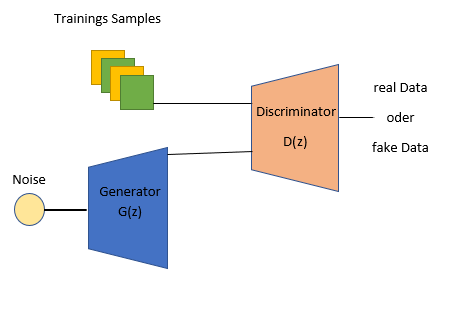
\includegraphics[width=0.5\textwidth]{GAN_GRUNDAUFBAU.png}
	\caption{Generativ Adverserial Network}
	\label{fig:Bild20}
\end{figure}
\\
Der Discriminator ist definiert durch D(x;$\Phi$\textsubscript{d}). Wobei $\Phi$\textsubscript{d} die Gewichte des Descriminators sind und D(x) die Wahrscheinlichkeit ist, dass x von den Trainingsdaten stammt und nicht von p\textsubscript{g}. Die Wahrscheinlichkeitsverteilung für unsere Trainingsdaten ist p\textsubscript{r}.  Im Training werden dann $\Phi$\textsubscript{d} so angepasst, dass die Wahrscheinlichkeit Trainingsbeispiele richtig zu klassifizieren maximiert wird. Und $\Phi$\textsubscript{g} wird dahingehen trainiert die Wahrscheinlichkeit zu minimieren, so dass D erkennt dass Trainingsdatensatz x von G erzeugt wurde. Mathematisch ausgedrückt durch log(1 - D(G(z))). Die gesamte Loss-Funktion des vanilla GAN ist definiert als:
\\\\
\begin{math}
min\textsubscript{G} max\textsubscript{D}V(D,G)=E\textsubscript{x$\sim$p\textsubscript{data}(x)}[logD(x)]  + E\textsubscript{z$\sim$p\textsubscript{z}(z)}[log(1-D(G(z))]
\\\\             
\end{math}
diese beschreibt ein Minmax Spiel zwischen G und D. Welches das globale Optimum erreicht hat wenn p\textsubscript{g} = p\textsubscript{r}. Das heißt, wenn die Datenverteilung, welche von G erzeugt wird, gleich der unserer Trainingsdaten ist\cite{goodfellow2014}. Das Training erfolgt durch den folgenden Algorithmus:
\\
\begin{algorithm}[H]
	\For{Anzahl von Training Iterationen}{\For{k Schritte}{$\bullet$Sample minibatch von m noise  Samples z\textsuperscript{(1)},...,z\textsuperscript{(m)}von noise p\textsubscript{g}(z)\\
	$\bullet$ Sample minibatch von m Beispielen x\textsuperscript{(1)},...,x\textsuperscript{(m)}von Daten Generationsverteilung p\textsubscript{data}(x)\\
    $\bullet$ Update den Discriminator zum aufsteigenden stochastischen Gradianten:\\
\begin{math}
\nabla\textsubscript{$\Phi$\textsubscript{d}}\frac{1}{m}\sum_{i=1}^{m}[logD(x\textsuperscript{(i)})+log(1-D(G(z\textsuperscript{(i)})))]
 \end{math}

}$\bullet$ Sample minibatch von m noise Samples z\textsuperscript{(1)},...,z\textsuperscript{(m)} von noise p\textsubscript{g}(z)\\$\bullet$ Update den Generator mit den absteigenden stochastischen Gradianten: \\\begin{math} 
\nabla\textsubscript{$\Phi$\textsubscript{g}}\frac{1}{m}\sum_{i=1}^{m}log(1-D(G(z\textsuperscript{(i)})))\end{math}}
		\caption{Minibatch stochastic gradient descent Training für Generative Adversarial Networks. Die Anzahl der Schritte welche auf den Discriminator angewendet wird ist k }	
\end{algorithm}

Beim Training wird ein stochastischer Minibatch von mehren Trainingsdaten gleichzeitig erstellt. Dies soll dabei helfen, dass der Generator sich nicht auf bestimmte Gewichte fest fährt und auf Trainingssätze kollabiert. So weisen die erzeugten Daten mehr Variationen auf \cite{improvingan}. D wird zunächst in einer inneren Schleife auf n Trainingsätzen trainiert, womit man Overfitting von D vermeiden will, was zur Folge hätte, dass D nur den Trainingsdatensatz kopieren würde. Deshalb wird k mal D optimiert und ein mal G in der äußeren Schleife. 
\\\\
Ein möglicher Aufbau von GAN wird in Abb. \ref{fig:Bild21} dargestellt. Dies ist das sogenannte Deep Convolution GAN(DC GAN), welches dafür konzipiert wurde auf Bilddaten zu arbeiten. Dabei besteht der Generator aus mehren Schichten von Deconvolution-Layern. Welche den Input Noise Variable p\textsubscript{z}(z) auf y abbildet. D besteht aus mehren Schichten von Convolution-Layern und bekommt als Input die Trainingsdaten, oder die von G erzeugten Y, und entscheidet über die Klassifikation\cite{dcgan}.
\begin{figure}[htbp] 
	\centering
	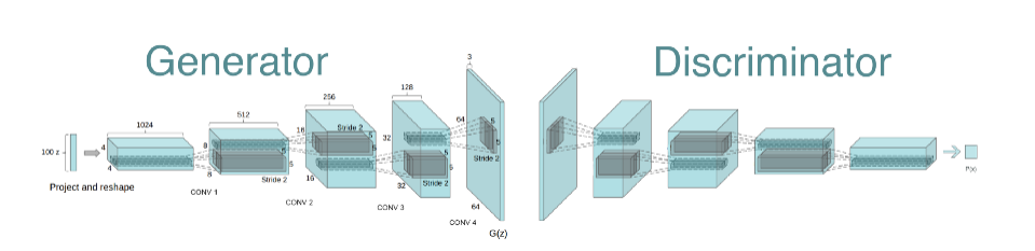
\includegraphics[width=1.0\textwidth]{dcgan1.png}
	\caption{Deep Convolutional GAN\protect\cite{dc-gan_book}}
	\label{fig:Bild21}
\end{figure}
Das asymmetrische Verhalten der KV Divergenz zu schlechten Trainingsergebnissen führt, welches von üblichen generativen Modellen wie Autoencoder verwendet wird. Goodfellow \cite{goodfellow2014} zeigte, dass sich die MinMax Loss-Funktion des GAN auch als Jensen-Shannon Divergenz(JS Divergenz) darstellen lässt. Diese ist definiert als:
\\\\
\begin{math} D\textsubscript{JS}(P\textsubscript{r}|| P\textsubscript{g}])=\frac{1}{2}D\textsubscript{KL}(P\textsubscript{r}|| \frac{P\textsubscript{g}+P\textsubscript{r}}{2}])+D\textsubscript{KL}(P\textsubscript{q}|| \frac{P\textsubscript{g}+P\textsubscript{r}}{2}])  
\end{math}
\\\\
wobei P\textsubscript{r} die Wahrscheinlichkeitsverteilung der Trainingsdaten ist und P\textsubscript{g} die des Generators. Huzár \cite{sha} zeigte, dass durch das symmetrische Verhalten der JS Divergenz ein potentiell besseres Trainingsergebnis entstehen kann, im Vergleich zu der KL Divergenz. Damit zeigte er weshalb GANs im Vorteil gegenüber anderen generativen Modellen sind.
\newpage
\subsubsection{Probleme mit GANs}\label{sec:problemegan}
~\\\\
Wie auch andere generative Modelle haben auch GANs noch Schwächen bezüglich der Trainingsabläufe und der Qualität ihrer generierten Daten. Im Folgenden wird auf einige Probleme eingegangen welche im darauffolgenden Kapitel Lösungs-ansätze aufgezeigt werden. 
\\
\begin{description}	
\item[Vanishing gradient]
~\\
Dies beschreibt das Problem, wenn D perfekt trainiert ist weil die beiden Datenverteilungen p\textsubscript{r} und  p\textsubscript{g} disjunkt sind. Und es keine Überschneidung der Datenverteilungen gibt.  Die Loss-Funktion würde in diesem Fall auf 0 fallen und es gäbe keinen Gradianten, für den die Gewichte von G angepasst werden können. Dies verlangsamt den Trainingsprozess bis hin zu einem kompletten Stopp des Trainings. Würde D zu schlechten trainieren mit D(x) = 0 für p\textsubscript{r} und  D(x) = 1 für p\textsubscript{g}. Bekommt G kein Feedback über seine Leistung bei der Datengeneration und hat keine Möglichkeit p\textsubscript{r} zu erlernen \cite{vanishing}.
\\
\item[Equilibrium]
~\\
D und G betreiben ein MinMax Spiel. Beide versuchen das Nash Equilibrium zu finden. Dies ist der bestmögliche Endpunkt in einen nicht kooperativen Spiel. Wie in dem Fall von GAN wäre das wenn  p\textsubscript{g} = p\textsubscript{r}. Es wurde gezeigt, dass das Erreichen dieses Punktes sehr schwierig ist, da durch die Updates der Gewichte mit den Gradianten der Loss-Funktion starke Schwingungen der Funktion enstehen können. Dies kann zu einem instabilen Orbit für das laufende Training führen \cite{improvingan}.   
\\
\item[Mode Collapse]
~\\
Ein weiteres Problem kann passieren wenn der Generator während des Trainings, auf ein bestimmtes Setting seiner Gewichte festhält und er bei der Datengeneration sehr ähnlichen Samples generiert. Dieses Problem wird Mode Collapse genannt\cite{improvingan}.
\end{description}

\subsubsection{Lösungsansätze für die GAN Probleme}
~\\\\
Nun werden einige Techniken aufgezeigt, welche die unter Abschnitt Probleme mit GAN genannten Schwierigkeiten angehen und zu einem effizienteren Training führen, damit eine schnellere Konvergenz während des Trainings erreicht wird.
\\
\begin{description}
\item[Feature matching]
~\\
Dies soll die Instabilität von GANS verbessern und gegen das Problem des Vanishing Gradient angehen. G bekommt eine neue Loss-Funktion und ersetzt die des üblichen Vanilla GAN. Diese soll G davon abhalten, sich an D über zu trainieren und sich zu sehr darauf zu fokussieren, D zu täuschen und gleichzeitig auch versuchen die Datenverteilung der Trainingsdaten abzudecken \cite{improvingan}.\\

\item[Minibatch discrimination] 
~\\
Um das Problem des Mode Collapse zu umgehen, so dass es nicht zu einem Festfahren der Gewichten von G kommt, wird beim Trainieren die Nähe von den Trainingsdatenpunkten gemessen. Anschließend wird die Summe über der Differenz aller Trainingspunkte genommen und dem Discriminator als zusätzlicher Input beim Training hinzugegeben \cite{improvingan}.\\

\item[Historical Averaging]
~\\
Beim Training werden die Gewichte von G und D aufgezeichnet und je Trainingsschritt verglichen. Anschließend wird an die Lossfunktion je Trainingschritt die Veränderung zu dem Trainingschritt davor an die Loss-Funktion addiert. Damit soll verhindert werden dann das Model sich zu sehr von seinen vorherigen Zustand der Gewichte entfernt. \cite{improvingan}.\\

\item[One-sided Label Smoothing]
~\\
Die üblichen Label für den Trainingsdurchlauf von 1 und 0 werden durch die Werte 0.9 und 0.1 ersetzt. Dies führt zu besseren Trainingsergebnissen. Es gibt derzeit nur empirische Belege für den Erfolg, jedoch nicht weshalb diese Technik besser funktioniert\cite{improvingan}.\\

\item[Wasserstein-GAN]
~\\
Die Wasserstein Metrik, oder auch Earth Mover Distance(EMD) genannt misst die Minimum Kosten welche entstehen wenn man Daten von der Datenverteilungp p\textsubscript{r} zur Datenverteilung p\textsubscript{g} überträgt. Es wird oft auch von "Masse" oder "Fläche" gesprochen, welche von p\textsubscript{r} zu p\textsubscript{g} getragen wird. Definiert ist sie durch:
\\\\
\begin{math} 
$
W(p\textsubscript{r},p\textsubscript{g})=$\inf_{\gamma\sim\prod(P\textsubscript{r},P\textsubscript{g})}$E\textsubscript{(x,y)$\sim\gamma$}[$\parallel$x - y$\parallel$]
$
\end{math}
\\\\
p\textsubscript{r} steht für die reale Datenverteilung zu welche uns Daten im Form von Trainingsdaten zur Verfügung stellen und p\textsubscript{g} steht für die generierte Datenverteilung, welche von einem Model erzeugt wird. Dabei wird nun das Infinum von allen möglichen Transportplänen $\gamma$, welche in $\prod$ enthalten sind ausgewählt, was der kostengünstigste Plan ist, die Daten von x zu y zu übertragen. Die EMD sind nun die Kosten von einem optimalen Transportplan. Vorteile sind unter anderem, dass der Gradient gleichmäßiger ist und das WGAN lernt besser auch wenn der Generator schlechtere Daten erzeugt im Vergleich zum üblichen GAN\cite{wasser}. Durch die Kantorovich-Rubinstein Methode kann die Wasserstein-Distanz umgeformt werden in zu:
\\\\
\begin{math} 
$
W(p\textsubscript{r},p\textsubscript{$\theta$})=$\sup_{\parallel f \parallel \textsubscript{L}\leq 1}$ E\textsubscript{x$\sim$P\textsubscript{r}}[f(x)] - E\textsubscript{x$\sim$P\textsubscript{$\theta$}}[f(x)]
$
\end{math}
\\\\
Durch diese Umformung ist es nun möglich, dass GAN die EMD nutzt um die von G generierten Daten mit den realen Daten zu vergleichen. Dabei übernimmt der Discriminator nun die Aufgabe eines Critic, welcher nun nicht mehr 0 oder 1 für Fake oder Real ausgibt sondern, einen Score, welcher angibt wieviel Masse von der P\textsubscript{$\theta$} also der Generator, umverteilt werden muss damit dieser bessere Ergebnisse liefert. Das Wasserstein GAN liefert bis dahin die erfolgreichste Verbesserung zum üblichen Vanilla-GAN von Goodfellow und erlaubt es, gegen die in Kapitel \ref{sec:problemegan} aufgezeigten Probleme Vanishing gradient und Model Collapse anzugehen\cite{wasser}. 
\end{description}
\newpage
\subsection{Conditional-GAN}\label{sec:cgan}

Conditional-GAN(C-GAN) ist eine Modifikation des ursprünglichen GAN von Goodfellow, welches erlaubt bedingte Wahrscheinlichkeiten in Datensätze zu erlernen. Das heißt zusätzliche Informationen in den Lernprozess einzuspeisen um den Output zu modifizieren. Im ursprünglichen GAN gibt es keine Möglichkeit auf den Output des Generators Einfluss zu nehmen. Dabei wird das Modell so verändert das eine zusätzliche Information y als Input in den Discriminator und Generator zugefügt wird. Dabei kann y jegliche Information sein wie Label, Bilddaten oder 3D-Daten. Dementsprechend muss die Zielfunktion dahin gehend angepasst werden bedingte Wahrscheinlichkeiten zu lernen
\\\\
\begin{math}
min\textsubscript{G} max\textsubscript{D}V(D,G)=E\textsubscript{x$\sim$p\textsubscript{data}(x)}[logD(x|y)]  + E\textsubscript{z$\sim$p\textsubscript{z}(z)}[log(1-D(G(z|y))]          
\end{math}
\\\\

\begin{figure}[htbp] 
	\centering
	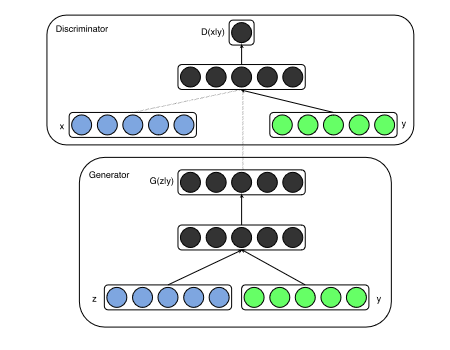
\includegraphics[width=0.5\textwidth]{cgan.png}
	\caption{Conditional Adverserial Network\protect\cite{cgan}}
	\label{fig:Bild38}
\end{figure}
Im Abb. \ref{fig:Bild38} kann der Informationsfluss und die Konnektivät der einzelnen Module entnommen werden. Die Module Generator und Discriminator bleiben gleich und können von ihrem Aufbau für die jeweiligen Datentyp verändert werden und Beispielsweiße durch Convolutional-Layer, Deconvolutional-Layer oder Fully-Connected-Layer bestehen\cite{cgan}.
\newpage
\subsection{3D-GAN}\label{sec:3dgan}

Das besondere am 3D Raum im Vergleich zu normalen 2D Bildern ist die Steigerung der Dimension und zu gleich der hohe Informationsgehalt welcher in 3D Objekten steckt. Das Ziel von 3D-GAN ist es die Datenverteilung der zugrunde liegenden 3D-Modellen zu erlernen. Dabei wird der latente Objektraum erfasst und soll dadurch die Wahrscheinlichkeiten für einzelne Objektklassen enthalten. 
\\\\
Es wurden schon mehrere Versuche von generativen Modellen auf 3D Daten durchgeführt wie von Wu, Jiajun und Zhang \cite{3d} welche in ihren Modell mit mit 3D-Voxel Daten arbeiten und damit ein GAN trainiert haben.Auch Achlioptas, Panos und Diamanti\cite{3dgan} welche ein GAN auf Punktwolken trainiert. Da in folgender Arbeit die 3D-Daten durch Punktwolken dargestellt werden wird die Arbeit von Achlioptas, Panos und Diamanti näher beleuchtet.
\\\\
Die Architektur des typischen 3D-GAN oder auch RAW-GAN betitelt ist dem Vanilla GAN von Goodfellow ähnlich. Der Input Layer ist ein Fully-Connected Layer welcher der Anzahl der Punkte je Punktwolke * 3 entspricht. Dieser bekommt als Input einen Noise-Vektor welcher aus einer Normal Verteilung entnommen wird und durch mehrere Layern gereicht bis hin zum Output Layer welche die Anzahl der gewünschten Punkte besteht. Also Zielfunktion kann mit der KL-Zielfunktion gearbeitet werden oder mit der Wasserstein Metrik welche im Versuchsaufbau von Achlioptas, Panos und Diamanti besser Ergebnissee geliefert hat. Der Aufbau unterscheidet sich nicht von Vanilla-GAN\cite{3dgan}. 

\begin{figure}[htbp] 
	\centering
	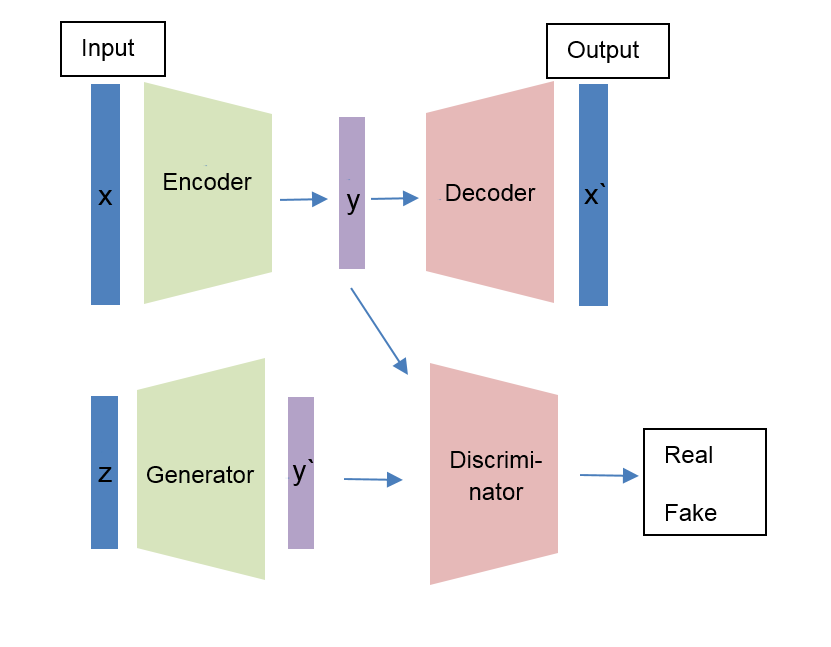
\includegraphics[width=0.5\textwidth]{latentgan.png}
	\caption{Latent-GAN}
	\label{fig:Bild39}
\end{figure}
~\\\\
Eine weitere Möglichkeit ist das Latent-GAN, dieses benutzt eine andere Aufbau gegenüber dem RAW-GAN, welches dabei helfen soll den latenten Raum der Objekte zu erlernen. Zunächst wird ein Autoencoder mit den vorhanden Trainingsdaten(vgl. \ref{sec:autoencoder}) trainiert. Der Aufbau ist der selbe einen üblichen 3D-Autoencoder beschrieben in Kapitel \ref{sec:autoencoder}. Ziel dabei ist den latenten Raum der Trainingsdaten zu erlernen und eine Kompression der Daten um den Suchraum zu  welcher beim RAW-GAN durch die Inputdimension gegeben ist, zu verringern und dadurch das Training des GANs zu erleichtern\cite{3dgan}. 
\\\\
Bevor das Training des Latent-GAN beginnen kann werden nun die Trainingsdaten durch den vorher trainierten Encoder des 3D-Autoencoder auf die festgelegte Output-Dimension komprimiert. Anschließend werden diese komprimierten Daten verwendet um das GAN zu trainierten. Dabei erlernt das GAN komprimierten Code zu produzieren, welcher anschließend durch den Decoder des 3D-Autoencoder wieder auf die ursprüngliche Größe gebracht werden kann. Durch dieses Verfahren war es möglich Daten in einer guten Qualität zu produzieren und eine Datenverteilung des zugrundeliegenden Models zu erlernen. Der gesamte Ablauf kann in Abb. \ref{fig:Bild39} entnommen werden\cite{3dgan}. 

\subsection{Rekonstruktion von Daten}\label{sec:rekdaten}

Derzeit setzt Deep Learning neue Maßstäbe bei der Rekonstruktion von Daten, wie Bildern oder Texten. Bei der Rekonstruktion geht es darum Daten, welche von ihren Urzustand verändert wurden, sei es durch Artefakte oder manuelle Bearbeitung, wieder dahin zurück geführt werden. In Abb. \ref{fig:Bild40} ist eine Rekonstruktion eines Bildes dargestellt welches eine Wiederherstellung eines Hundes zeigt. Deep Learning hat in diesem Bereich besonders bei Bilder große Erfolge erzielt. Da diese als Matrizen dargestellt werden können, liefern sie eine Datenstruktur, auf welche KNN arbeiten können. Auch Bearbeitung mit Convolutionen-Layer auf Bilddaten zählt als Erfolg für die Weiterverarbeitung\cite{imagerecon}. Durch die genannten Methoden werden bessere Strukturen für das jeweilige Ziel, in diesem Fall die Rekonstruktion, gelernt und ermöglicht es wie in verschieden Papern wie \cite{imagere1}  welche auf super-hochauflösenden Bildern Artefakte entfernt und das Bild wieder zum Urzustand zurück führt.
\\\\
Auch wie die Arbeit von Liu, Gulin und Reda \cite{imagere2} konnte ähnliche Ergebnisse liefern. Rekonstruktion auf 3D-Daten wurde von Yi, Li und Shao \cite{3d_recon} durchgeführt. Diese Arbeiteten beinhaltet jedoch die Rekonstruktion von 2D Bildern auf 3D Modellen. Dabei wurde mit Hilfe von Autoencoder gearbeitet was auch für die folgenden Arbeit von Bedeutung sind\cite{3d_recon}. Da diese helfen durch die Dimensionreduktion eine einfachere Daten Weiterverarbeitung zu liefern. 

\begin{figure}[htbp] 
	\centering
	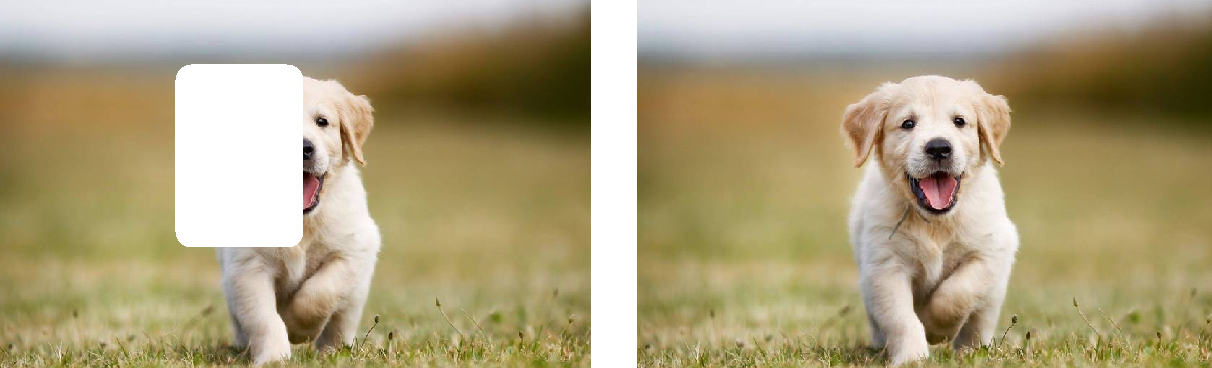
\includegraphics[width=0.6\textwidth]{imagere.png}
	\caption{Bild Rekonstruktion eines Hundes welches durch ein Artefakt zerstört wurde}
	\label{fig:Bild40}
\end{figure}
\newpage
\section{Methoden}
In diesem Kapitel werden die Methoden für die Versuchsaufbauten 1 und 2 aufgezeigt, welche die Fragestellungen 1 und 2 überprüfen sollen, die unten festgehalten wurden.
\begin{description}
	\item[Fragestellung 1]
	Können durch GANs 3D-Punktwolken von Tabakblättern erlernt werden um neue Datensätze zu generieren?\\
	
	\item[Fragestellung 2] Können durch GANs 3D-Punktwolken von Tabakblättern, die von ihrem Urzustand abgebracht wurden, rekonstruiert werden? 
\end{description}
Die Fragestellung beinhaltet ob mit Hilfe von GANs der latente Objektraum eines Tabakblattes gelernt werden kann und anschließend durch den Generator des GAN Tabakblätter erzeugt werden können. Dieser Versuchsaufbau wird in Kapitel \ref{sec:versuch1-aufbau} behandelt. Die dazugehörigen Trainingsdaten werden in Kapitel \ref{sec:versuch1-traingsdaten} vorgestellt. Bei Fragestellung 2 soll überprüft werden, ob es mit Hilfe von GAN möglich ist Artefakte, von Tabakblätter zu entfernen und den Urzustand wieder her zustellen.  Dieses Verfahren wurde in Kapitel \ref{sec:rekdaten} beschrieben. Die Trainingsdaten für diesen Versuchsaufbau können Kapitel \ref{sec:versuch2_daten} entnommen werden. 
\\\\
Versuchsaufbau 1.2 und 2.1 wurden auf einem Computer mit Ubuntu 14.05 Betriebssystem mit einen IntelR CoreTM i7-7700k mit 4.50GHz einer Geforce GTX 1080 mit 8G Grafikspeicher durchgeführt. Training und Test  wurden mit CUDA 9.0 und cudNN 7.1.1. Als Programmiersprache wurde Python 2.7 bzw. 3.5 für Datengenerierung verwendet. Als ANN Libary wurde Tensorflow 1.5 genutzt und TFlearn 0.3.2. Für die EMD und Chamfer Loss des Autoencoder wurde die Implementierung von dfanhqme (https://github.com/fanhqme/PointSetGeneration) benutzt.
\\\\
Versuchsaufbau 1.1 und 2.2  wurden auf einen Computer mit Windows Betriebssystem mit einen IntelR CoreTM i7-7700k mit 4.50GHz einer Geforce GTX 1080 mit 8G Grafikspeicher durchgeführt. Training und Test wurden mit CUDA 9.0 und cudNN 7.1.1 durchgeführt. Also Programmiersprache wurde Python 3.5 verwendet. Als ANN Libary wurde Tensorflow 1.10 genutzt.
\newpage

\subsection{Datensatz 1. Versuchsaufbau}\label{sec:versuch1-traingsdaten}
~\\\\
Der erste Datensatz ``Stühle`` besteht aus 6778 Punktwolken, mit jeweils 2048 Punkten. Dieser wurde dem Shapenet Datensatz(www.shapenet.org) entnommen. Die Daten sind im PLY Datenformat abgespeichert. Ein Beispielpunktwolke kann aus Abb. \ref{fig:Bild50} entnommen werden. Der Datensatz wurde auch in der Arbeit von Achlioptas, Diamanti, Mitliagkas und Guibas\cite{3dgan} verwendet, was Kapitel \ref{sec:3dgan} bereits vorgestellt wurde ist. In der hier liegenden Arbeit dient er als Validierungsdatensatz, um die Qualität der generierten Daten des GAN, welches mit Tabakblättern trainiert wurde, zu vergleichen.
\\\\
Die Daten für den zweiten Datensatz ``Blätter`` stammen vom Fraunhofer-Institut und deren Gewinnung wurde in Kapitel \ref{sec:punktwolken} beschrieben. Der Grunddatensatz bestand aus mehreren 3D-Scans von Tabakpflanzen, bei den die Blätter der Pflanze zu einem Datensatz zusammengefügt wurden. Der "Blätter" Datensatz besteht aus 422 Punktwolken welche, dann durch ein Punktreduktionsverfahren auf jeweils 2048 Punkten je Punktwolke reduziert worden ist. Aus Komplexitätsgründen wurden der Farbchannel in dieser Arbeit außen vor gelassen, um den Informationsgehalt der Daten zu reduzieren und ein Training zu vereinfachen. Außerdem spielen Farben beim derzeitigen Ziel der Arbeit, Rekonstruktion von Tabakblättern keine Rolle und nehmen keinen Einfluss auf die Verwendbarkeit des Ergebnisses. Abgespeichert werden die Daten im PLY-Datenformat.

\begin{figure}[htbp] 
	\centering
	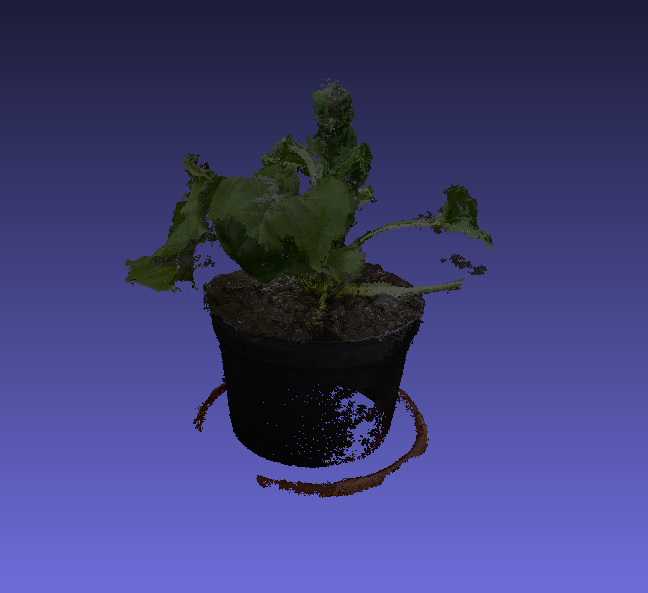
\includegraphics[width=0.6\textwidth]{plant.png}
	\caption{3D Punktwolke einer Tabakpflanze}
	\label{fig:Bild50}
\end{figure}

\begin{figure}[htbp] 
	\centering
	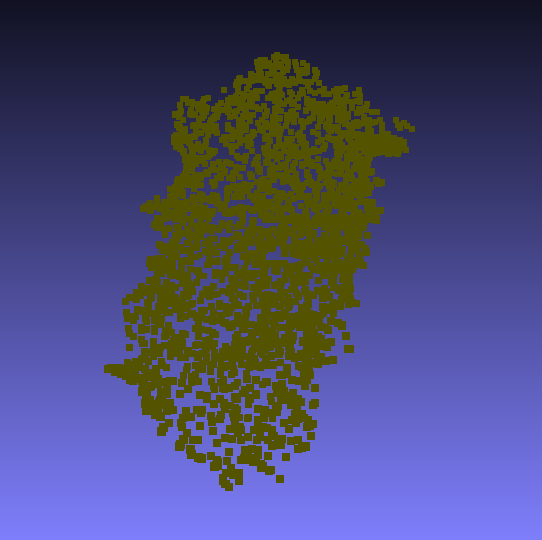
\includegraphics[width=0.5\textwidth]{leaf1.png}
	\caption{3D Punktwolke eines Tabakblattes mit 2048 Punkten}
	\label{fig:Bild51}
\end{figure}
\newpage
\subsection{Datensatz 2. Versuchsaufbau}\label{sec:versuch2_daten}

Für den zweiten Versuchsaufbau wird auf den in Datensatz Versuchsaufbau 1. Blatt Datensatz ``Blätter`` zurück gegriffen. Der Grunddatensatz besteht aus 422 unterschiedlichen Blättern. Dieser Datensatz wird nun dahingehen verändert, das Löcher in die Blattoberfläche eingefügt werden. Diese Löcher simulieren das andere Blätter bei dem Scanverfahren die Sicht des Scanners auf das Blatt verdecken und dieses somit unvollständig eingescannt wird. Dieses Verdecken wir durch 3D-Sphären simuliert wie in Abb. \ref{fig:Bild52}  rot dargestellt. Die Sphären bestehen aus 10 000 Punkten, welche alle einen maximalen Radius von 15 mm haben und alle aus einer Normalverteilung entnommen werden, um  eine gleichmäßige Verteilung der Punkte zu gewährleisten. Die Sphären werden nun vom Koordinatenursprung im euklidischen Raum bewegt, sodass sich 46 unterschiedliche Sphären im Raum ergeben. Diese werden dahin gehend im Raum bewegt um möglichst eine hohe Differenzmenge mit den 422 Blättern im Datensatz zu haben. In Abb. \ref{fig:Bild53} sind alle Sphären symbolisch eingefügt, um dieses Vorgehen zu Veranschaulichen. Um nun das Verdecken zu simulieren, wird die Differenzmenge je Blatt mit einer der Sphären errechnet. Wobei die Differenzmenge eines Punktes der nächste Nachbar in einen Radius von 3mm befindet. Durch die dieses Verfahren entstehen kreisförmige Löcher in den Blättern welches in Abb. \ref{fig:Bild54} dargestellt ist. Anschließend werden alle erzeugten `` zerstörten`` Blätter nach der Anzahl ihrer übrig geblieben Punkte gefiltert um zu gewährleisten das genügen Punkte aus dem Urblatt entfernt worden sind und eine visuelle Diskrepanz zwischen den Blätter vorhanden ist. Dieses Vorgehen hat letztendlich zu 2047 zerstörten Blättern mit jeweils 2048 Punkten geführt.

\begin{figure}[htbp] 
	\centering
	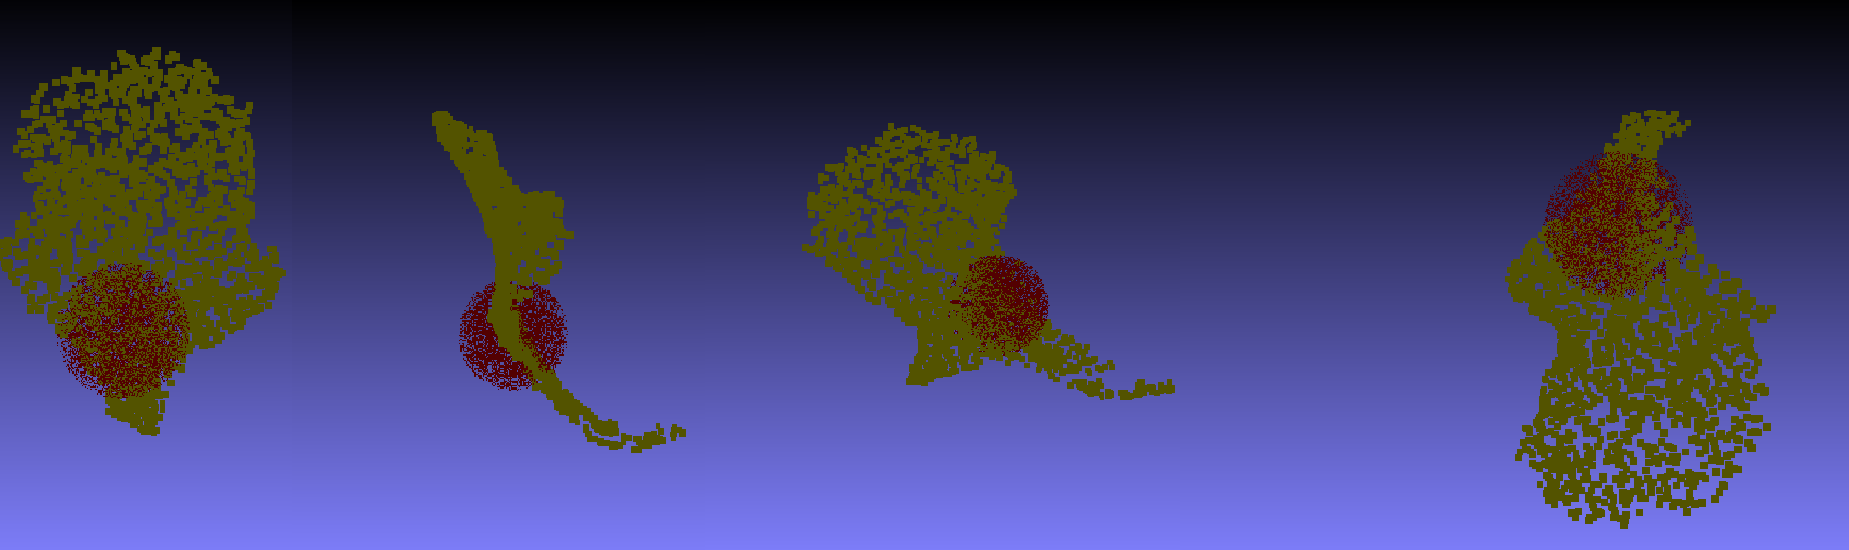
\includegraphics[width=1.0\textwidth]{sphere1.png}
	\caption{Tabakblatt mit Sphäre welche die Differenzmenge bilden}
	\label{fig:Bild52}
\end{figure}

\begin{figure}[htbp] 
	\centering
	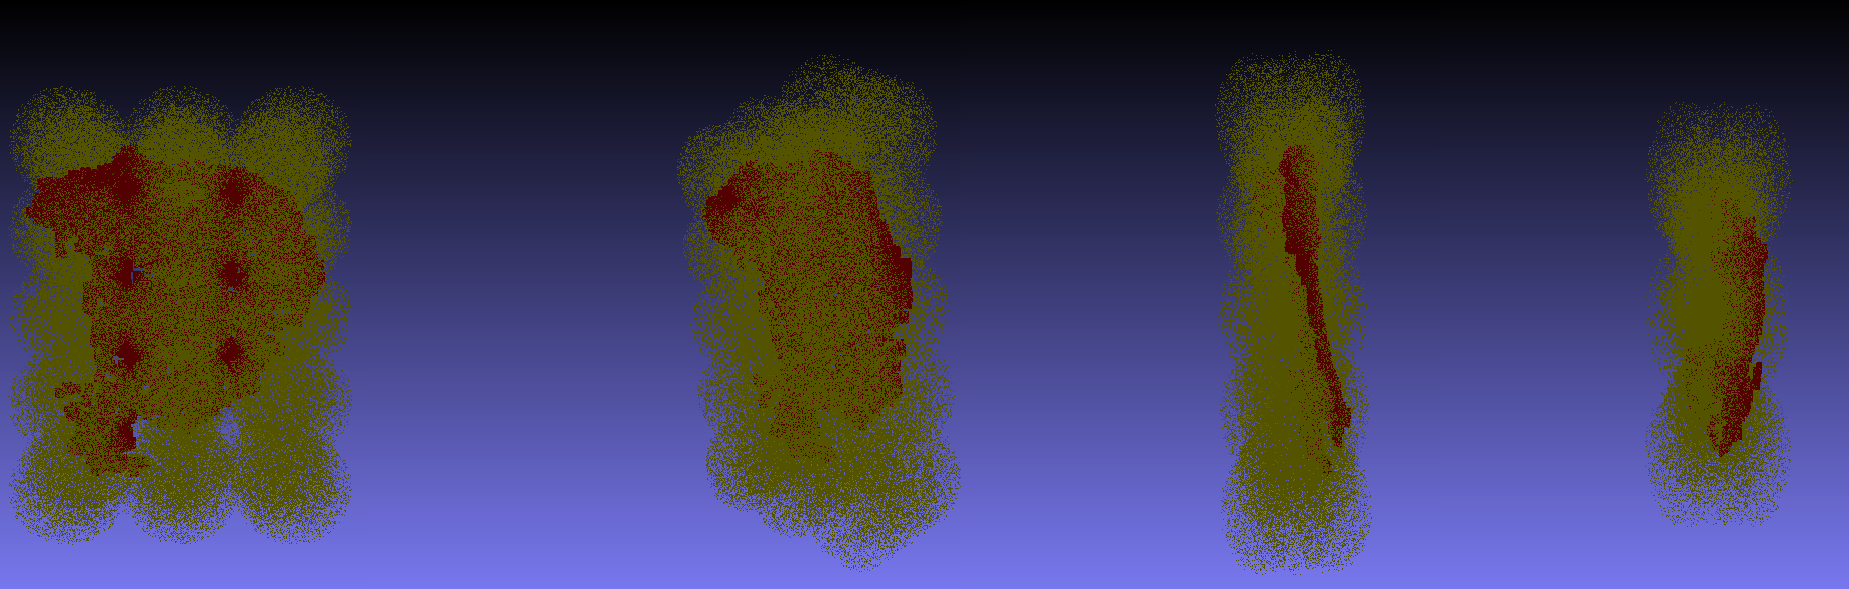
\includegraphics[width=1.0\textwidth]{allsphere.png}
	\caption{Sphäre im Raum welche das verdecken der Blätter simulieren}
	\label{fig:Bild53}
\end{figure}

\begin{figure}[htbp] 
	\centering
	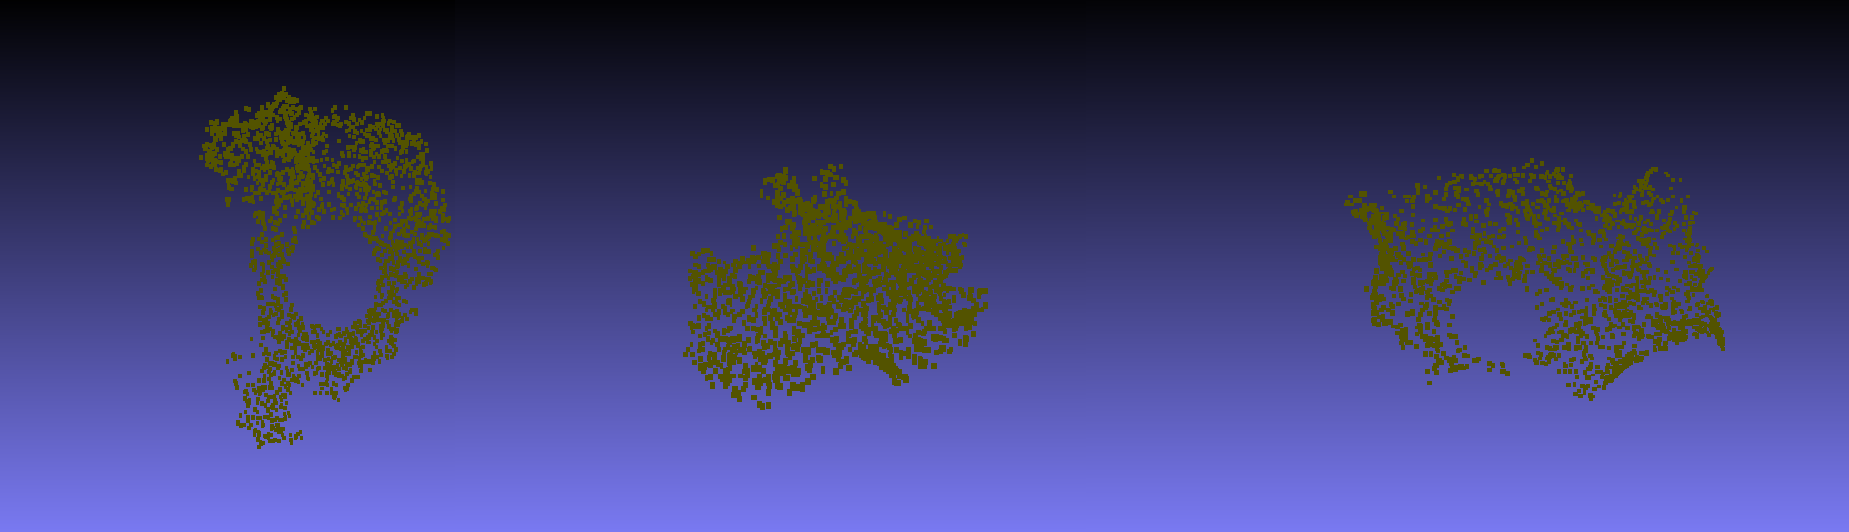
\includegraphics[width=1.0\textwidth]{training_destroyed.png}
	\caption{3D Punktwolke von zerstörten Tabakblättern}
	\label{fig:Bild54}
\end{figure}
\newpage


\subsection{Versuchsaufbau 1 - GAN}\label{sec:versuch1-aufbau}

Der Versuchsaufbau 1 besteht aus zwei unterschiedlichen Versuchen. Aufbau 1.1 ist das RAW-GAN(\cite{3dgan}), dabei wird auf den Vanilla-GAN Aufbau zurückgegriffen. Die Meta Trainingsvariablen für diesen Versuch sind Learningrate mit 0,0005 und einen Adam Optimizer, welcher zu den Mini-Batch Gradient Descent Verfahren aus Kapitel \ref{sec:test}, und dabei auf das aus Kapitel \ref{sec:momentum}, zurückgreift, mit einem Beta1 von 0,5 und einem Beta2 von 0,5. Die Batchgröße ist 64. Der Discriminator besteht aus 5-Layern, welche aus 1-Dimensionalen Convolutionen-Layer bestehen mit einer Filteranzahl [64, 128, 256, 256, 512] je Layer. Mit einer Kernel Größe von 1 und Stride von 1. Also Aktivierungsfunktion wird die ReLu-Funktion genutzt. Darauf folgen 3 Fully-Connected-Layer mit der Größe [128, 64, 1] alle mit einer ReLu-Funktion. Der Generator des RAW-GAN besteht auf 6 Fully-Connected-Layern mit [64, 128, 512, 1024 ,1536 ,6144] Neuronen, jeweils mit der Relu Aktivierungsfunktion. Der Noisevektor z wird aus einer 128-D Normal Verteilung entnommen mit $\mu$ = 0 und $\sigma$ =  0,2. Als Zielfunktion wird die Wasserstein Metric gewählt da diese bessere Ergebnisse im Versuchsaufbau von Achlioptas, Panos und Diamanti\cite{3dgan} erzielt hat. Das Training erfolgt jeweils mit den Datensätze "Stühle" und "Blätter" wie in Kapitel \ref{sec:versuch1-traingsdaten} beschrieben.
\\\\
Der Versuchsaufbau 1.2 ist das Latent-GAN, welches in Kapitel \ref{sec:3dgan} bereits vorgestellt wurde. Es wurde die Implementierung von \cite{3dgan} verwendet $(www.github.com/optas/latent_3d_points)$. Zunächst wird dabei der Autoencoder mit den Trainingsdaten trainiert. Das Training erfolgt mit einer Learningrate von 0,0005 und einer Batchsize von 50. Der Encoder besteht dabei aus 4 1-D Convolutional-Layern mit [64, 128, 246, 1024] Filtern, eine Stride von 1 und Size von 1. Die Batchgröße ist 64. Als Aktivierungsfunktion wir die Relu verwendet. Der Encoder besteht aus 3 Fully-Connected-Layern mit [256, 256, 6144] Neuronen, alle mit der ReLu-Zielfunktion. Das Training erfolgt jeweils mit den Datensätze "Stühle" und "Blätter" wie in Kapitel \ref{sec:versuch1-traingsdaten} beschrieben und wurde auf 500 Epochen durchgeführt. Nach dem Training des Autoencoder kann der komprimierte Latent Code welcher von Encoder erstellt wird, dazu verwendet werden, das Latent-GAN zu trainieren. Alle Trainingsdaten werden nun durch den Encoder komprimiert, um ihre 128-D Latenten Code y zu erzeugen. Mit diesen wird nun das GAN trainiert, um eigene Latente Codes zu produzieren, welche vom Decoder wieder auf ihre ursprüngliche Dimension von 2048 Punkten projiziert werden. In Abb. \ref{fig:Bild39} ist dieser Prozess dargestellt. Der Generator des Latent-GAN besteht aus 2 Fully-Connected-Layer mit [128, 128] Neuronen, welche als Aktivierungsfunktion eine ReLu-Funktion benutzen. Der Noisevektor z wird aus einer 128-D Normal Verteilung entnommen mit $\mu$ = 0 und $\sigma$ =  0,2. Der Discriminator besteht aus [128, 64, 1] Fully-Connected-Layern welche ebenfalls ReLu-Funktion nutzen. Als Zielfunktion wird die Wasserstein Metrik gewählt, da diese bessere Ergebnisse im Versuchsaufbau von Achlioptas, Panos und Diamanti\cite{3dgan} erzielt hat. 

\subsection{Versuchsaufbau 2 - CGAN für Punktwolkenrekonstruktion }\label{sec:versuch2-aufbau}

Da im Versuchsaufbau 1 das Latent-CGAN bessere Ergebnisse beim erlernen von Punktwolken Daten liefert, wird im Versuchsaufbau 2.1 Latent-CGAN das komprimieren von Trainingsdaten übernommen und dahin gehend verändert, dass Ziel von C-GAN zu übernehmen und bedingte Wahrscheinlichkeiten zu lernen. Zunächst werden wie bei Versuchsaufbau 1 die Trainingsdaten vgl.\ref{sec:versuch2_daten} an einen Autoencoder trainiert. Dabei wird jeweils ein Autoencoder für zerstörte Blätter heran genommen und einer für unzerstörte im Urzustand.
\\\\
Die Autoencoder folgen dabei den gleichen Aufbau wie in Versuchsaufbau 1.2. Der Encoder besteht dabei aus 4 1-D Convolutional-Layern mit [64, 128, 246, 1024] Filtern, eine Stride von 1 und Size von 1. Als Aktivierungsfunktion wird die ReLu-Funktion verwendet. Der Decoder besteht aus 3 Fully-Connected-Layern mit [256, 256, 6144] Neuronen, alle mit der ReLu-Zielfunktion. Als Batchsize wird 64 genommen. Als Zielfunktion wird jeweils einmal die CD getestet und die EMD. Für den Autoencoder wurde die Implementierung von \cite{3dgan} verwendet$(www.github.com/optas/latent_3d_points)$. 
\\\\
Der Generator des Latent-CGAN bekommt als Input z einen 128-D Vektor, welcher aus einer Normal Verteilungz mit $\mu$ = 0 und $\sigma$ =  0,2 entnommen wurde. Y welches zusätzlich zu z den Generator zum Training eingespeist wird sind die von Autoencoder codierten 128-D komprimierten zerstörte Tabakblätter. Der Generator des Latent-GAN besteht aus 2-Fully-Connected-Layer mit [128, 128] Neuronen, welche als Aktivierungsfunktion eine Leaky-ReLu-Funktion benutzen. Der Discriminator besteht aus 2 Fully-Connectected-Layern mit der Größe [128, 128]. Der Discriminator bekommt als Input entweder den vom Generator erzeugten latenten Code x' welcher vom Encoder des Autoencoder zu einen unzerstörten Blatt gemappt werden kann und zusätzlich y also (x',y). Oder ein aus unseren Trainingsdaten stammendes (x,y) Paar, welche als reale-Datensätze gekennzeichnet sind. Als Ziel wird jeweils die Wasserstein Metrik und die Vanilla - GAN Metrik Loss-Function benutzt. Beim Trainingsaufbau 2.2 RAW-CGAN bekommt der Generator als Input Noisevektor z einen 128-D Vektor, aus einer  Normal Verteilung entnommen mit $\mu$ =  0 und $\sigma$ =  0,2. Des weiteren wird als y den Generator die zerstörte Blatt Punktwolke welche als ein 6144-D Vektor dargestellt werden als Input übergeben. Der Generator besteht aus Fully-Connected-Layern mit [6272, 3163, 1568, 3136, 4850, 5680, 6144] Neuronen je Layer. Als Aktivierungsfunktion wird die Leaky-ReLu genommen. Im letzten Layern wird keine Aktivierungsfunktion verwendet um den Output linea verarbeitbar zu machen und damit Euklidische Koordinaten generiert werden können. Des weiteren wird nach jedem Layer ein Batch-Normalisation-Layer eingesetzt mit Momentum 0,9 und einen Beta1 und Beta2 von 0,5 eingesetzt. Des Discriminator besteht aus [12288, 6144, 3072,1536, 768, 384, 128, 32, 1] Fully-Connected-Layern mit Aktivierungsfunktion Leaky-ReLu bis auf den letzten Layer in den wird die Sigmoid-Funktion verwendet, wenn als Zielfunktion die Vanilla-GAN gewählt wird. Bei Verwendung der Wasserstein Metrik wird auf eine Aktivierungsfunktion verzichtet. Des weiteren wird nach jedem Layer ein Batch-Normalisation-Layer eingesetzt mit Momentum 0.9 und einen Beta1 und Beta2 von 0,5. Der Input des Discriminator ist die vom Generator erstellten (x',y) oder die direkt aus dem Trainingsdaten stammenden Punktwolken Paare des zerstörten Blatt y und Urzustand Blatt x als Tupel (x,y).Als Zielfunktion wird die Vanilla-GAN und W-GAN Zielfunktion getestet.
\\\\
Im weiteren Versuchsaufbau für den RAW-CGAN wird der Discriminator umgebaut um ihn durch Convolutional-Layer bessere Lernfähigkeiten zu geben. Dies sorgt nicht nur für Vorteile für den Discriminator dadurch kann auch der Generator durch den Gradianten des Discriminators einen besseren latenten Raum lernen. Der Generator bleibt in diesen Aufbau gleich der Discriminator bekommt [64, 128, 256, 256, 512] 1-D-Convolutional-Layer, mit einer Kernel-Größe von 1 und Stride von 1 als Aktivierungsfunktion wird eine Leaky-ReLu verwendet. Die Batchsize beträgt 64. Anschließend folgen [128, 32, 1] Fully-Conncected-Layer mit Leaky-Relu. Zwischen jeden Layer befindet sich ein Batch-Normalisation-Layer mit Momentum von 0,9 und einen Beta1 und Beta2 von 0,5. Abb. \ref{fig:Bild55} kann der Aufbau und Konnektivät der einzelnen Komponenten entnommen werden.

\begin{figure}[htbp] 
	\centering
	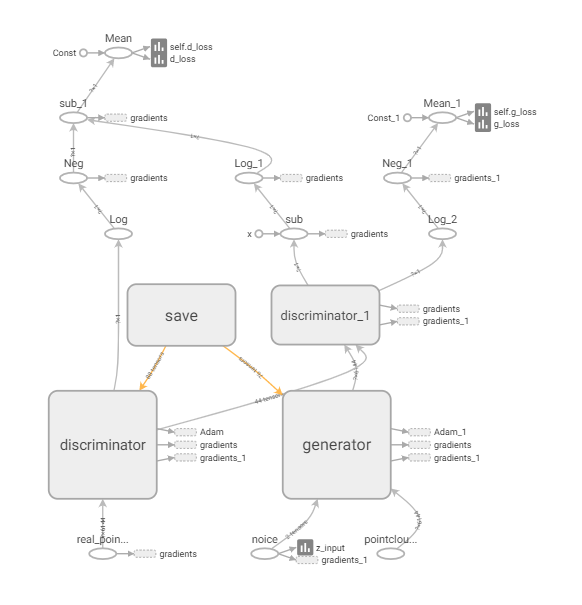
\includegraphics[width=0.7\textwidth]{point-cgan.png}
	\caption{Aufbau des RAW-CGAN}
	\label{fig:Bild55}
\end{figure}
\newpage

\section{Evaluation und Ergebnisse}

In diesen Kapitel wird auf die Ergebnisse von Versuchsaufbau 1 und 2 eingegangen. Zunächst wird Versuchsaufbau 1, vgl. \ref{sec:versuch1-aufbau} des Erlernen von latentem Raum von Punktwolken gezeigt. Dabei wird ein Vergleich zwischen den Modeldatensatz ``Stühle`` sowie einen aus der Praxis stammenden Datensatz ``Blätter`` aufgezeigt. Anschließend wird auf die Ergebnisse aus Versuchsaufbau 2 vgl. \ref{sec:versuch2-aufbau} eingegangen. Dabei wird evaluiert, ob es möglich ist die zerstörten Blattdaten in ihrem Urzustand wieder herzustellen und aussagekräftige Ergebnisse für die Anwendbarkeit in der Praxis vorhanden sind. Da es keine gängige Validierungsmethoden, beziehungsweise Validierungsmetriken gibt, wird sich bei der Prüfung der Testergebnisse auf das menschliche Auge verlassen, so dass die Prüfung in Form einer Sichtprüfung erfolgt.

\subsection{Ergebnisse - Versuchsaufbau 1}

Von RAW-GAN aus Versuchsaufbau 1.1 mit den Blattdaten lassen sich nach 500 Epochen Training Beispieldatensätze, welche vom Generator erzeugten wurden aus Abb.\ref{fig:Bild100} entnehmen. Wie zu erkennen ist, sind die Blätter nicht gut genug für eine Weiterverarbeitung. Der latente Raum, welcher von den GAN gelernt wurde und am Ende durch den Generator produziert wurde, zeigt keine Ähnlichkeit mit normalen Blättern, welche im Datensatz enthalten waren. Die Daten erinnern eher an einen hohlen Ball, als an Blättern. Es formen sich Punktansammlungen in der nähe des Koordinatenursprungs und es lässt sich kein Anzeichen von Bilden einer Blattfläche erkennen.
\begin{figure}[htbp] 
	\centering
	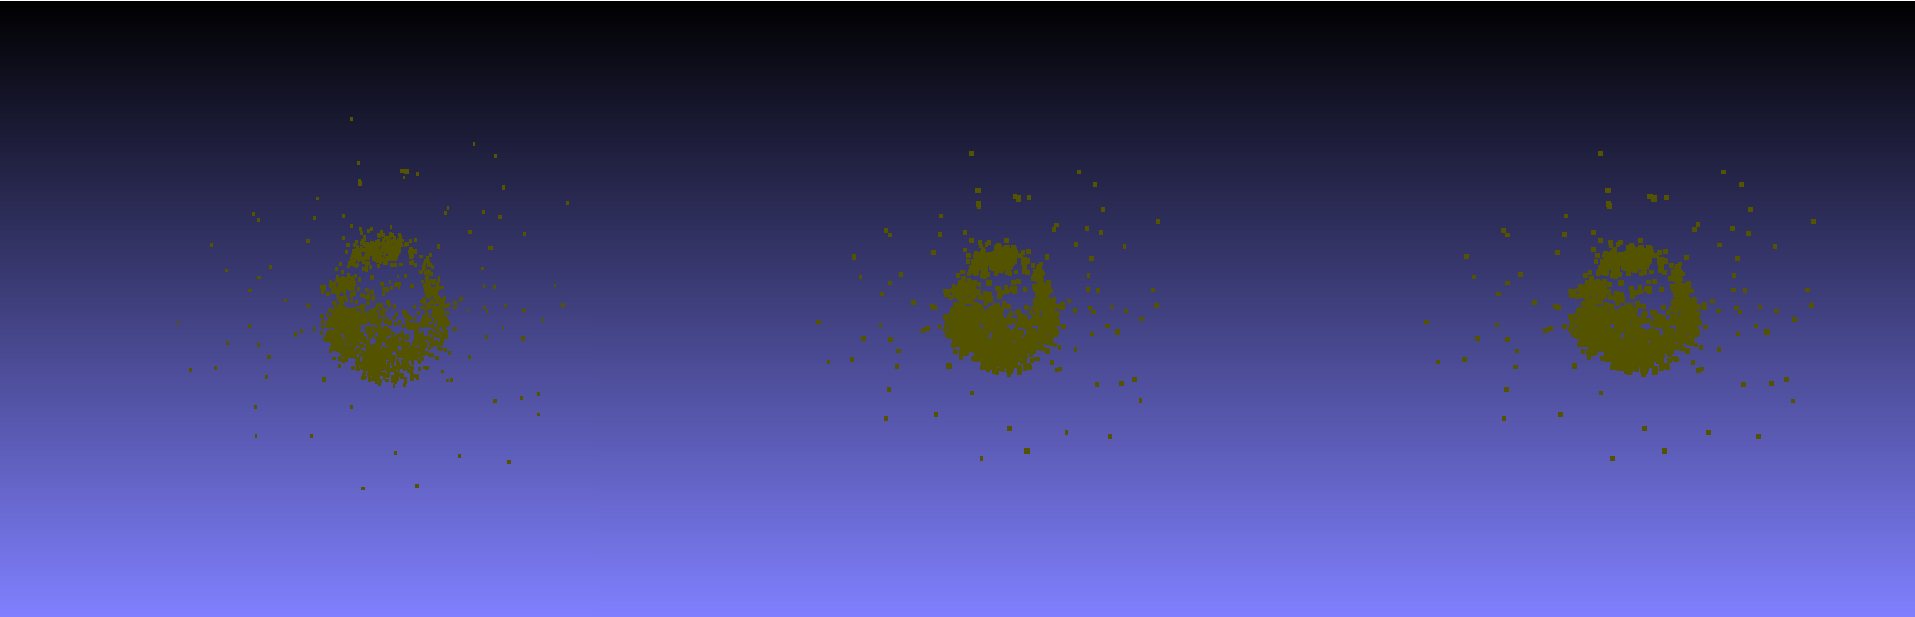
\includegraphics[width=1.0\textwidth]{raw_gan_leaf_example.png}
	\caption{Generierte Beispieldaten vom Generator des RAW-GAN mit den Blattdaten}
	\label{fig:Bild100}
\end{figure}
Die starke Punkthäufung am Koordinaten Ursprung ergeben sich dadurch, dass die realen Blattdaten an dieser Stelle häufig vertreten sind und sich an den Blattkanten eher unterscheiden. So lernt der Generator an diesen vermehrten Schnittpunkt mehr Punkte zu generieren als außerhalb. Dieser Effekt ist in Abb. \ref{fig:Bild81} zu erkennen. Dargestellt sind 24 Datensätze aus dem Blattdatensatz, welche aus verschiedenen Blickwinkeln in einen Koordinatensystem geladen wurden sind. Die Punkte häufen sich in der Nähe des Koordinatenursprungs und sind im äußeren Bereich schwächer Verteilt. 
\begin{figure}[htbp] 
	\centering
	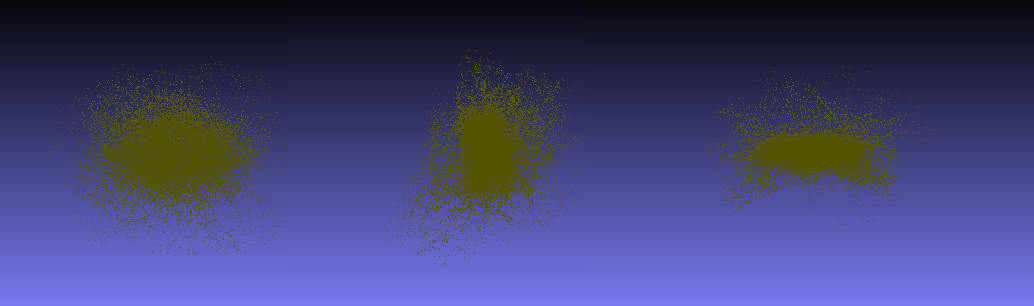
\includegraphics[width=1.0\textwidth]{ansammlung.png}
	\caption{24 Punktwolken aus dem Blattdatensatz in einen Koordinatensystem}
	\label{fig:Bild81}
\end{figure}
Vergleicht man dies mit Abb.\ref{fig:Bild100} sind dort dichte Ansammlungen ebenfalls zu erkennen. Der W-GAN Loss für den Generator und Discriminator kann in Abb. \ref{fig:Bild1002} entnommen werden. Der Loss des Discriminators konstant über mehrere Epochen bleibt, lässt sich daraus schließen, dass der Critic keine Schwierigkeiten hat die beiden Datenverteilungen zu Unterscheiden. Es ist kein Anzeichen von Verbesserung zu erkennen wenn das Training länger als 500 Epochen läuft. 
\begin{figure}[htbp]
	\centering
	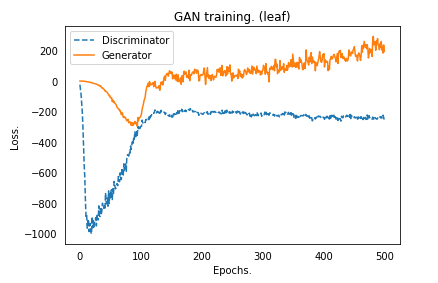
\includegraphics[width=0.5\textwidth]{raw_gan_leaf_result.png}
	\caption{Trainingsverlauf des RAW-GAN mit den Blattdaten}
	\label{fig:Bild1002}
\end{figure}
~\\\\
Ähnliche Ergebnisse sind auch beim RAW-GAN von Versuchsaufbau 1.1 mit den Stuhldaten zu beobachten. Wobei die Qualität der Stühle stärker an die im Trainingsdatensatz enthalten Daten erinnert vgl. Abb. \ref{fig:Bild58}. Es zeichnen sich Lehne und Stuhlbeine in den Daten ab, die vom GAN trainierten Generator stammen. Der Trainingsverlauf ist Abb. \ref{fig:Bild57} zu entnehmen. Dabei ist zu sehen das der Discriminator sich nicht mehr verbessert und der Generator keine besseren Ergebnisse liefern kann. Diese Ergebnisse decken sich mit den von Achlioptas, Panos und Diamanti \cite{3dgan} festgestellten Ergebnissen in den das RAW-GAN keine qualitativ gute Stuhldaten erzeugen konnte. 
\begin{figure}[htbp] 
	\centering
	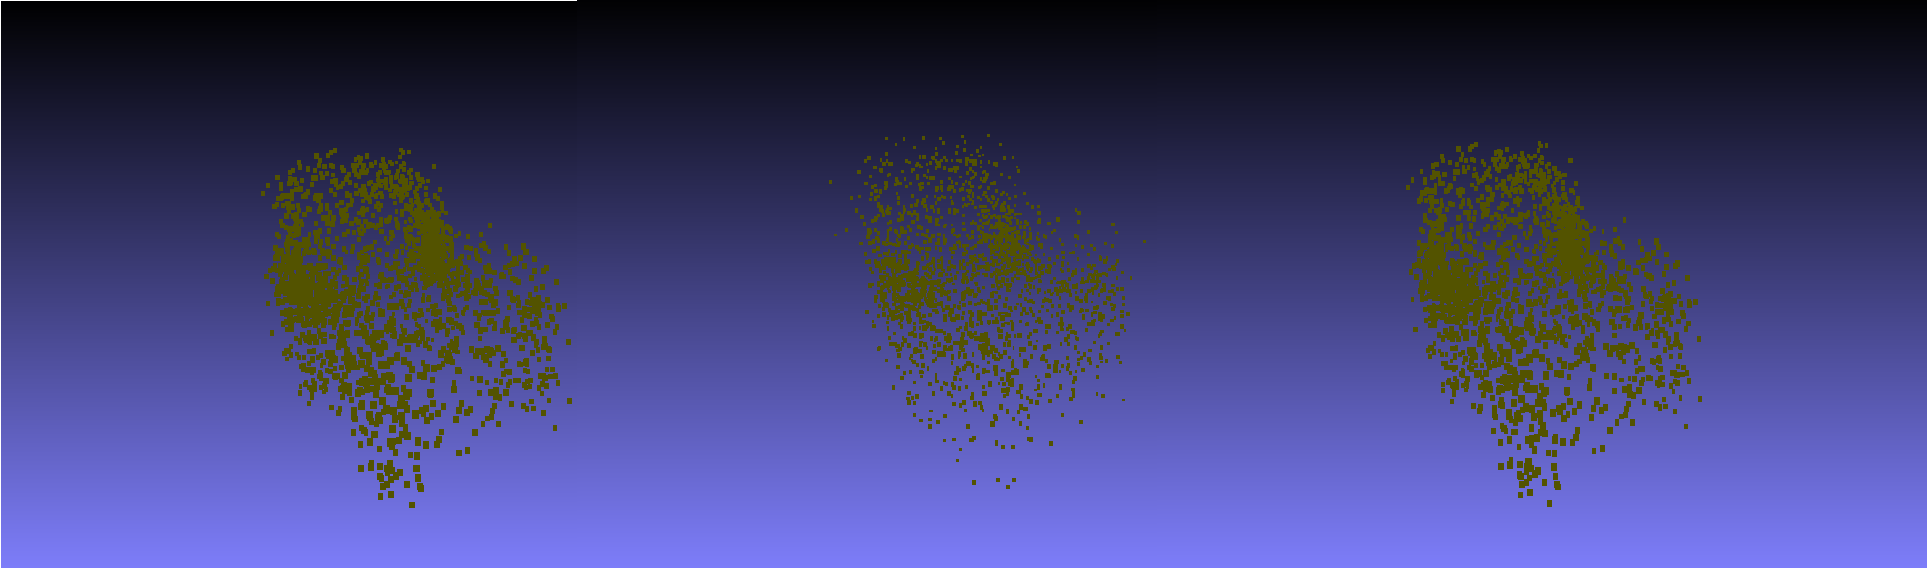
\includegraphics[width=1.0\textwidth]{raw_gan_chair_example.png}
	\caption{Generierte Beispieldaten von Generator des RAW-GAN mit den Stuhldaten}
	\label{fig:Bild58}
	\end{figure}
\begin{figure}[htbp] 
	\centering
	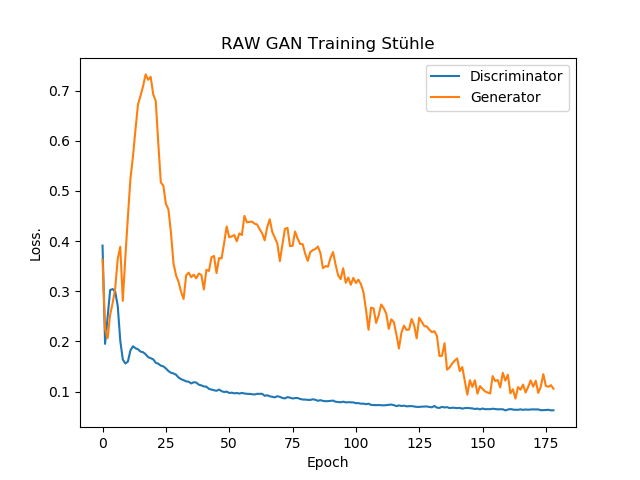
\includegraphics[width=0.5\textwidth]{raw_gan_chair_result.png}
	\caption{Trainingsverlauf des RAW-GAN mit den Stuhldaten}
	\label{fig:Bild57}
\end{figure}
\pagebreak\linebreak 
Um nun die Ursache genauer zu beleuchten, was die Gründe für  den Qualitätsunterschied zwischen den beiden generierten Datensätzen ausmacht und um festzustellen ob durch mehr Blattdaten bessere Ergebnisse erzeugt werden können, wurden die Stuhldaten auf 422 Trainingsdaten reduziert und ein erneutes Training des RAW-GAN durchgeführt. Die erzeugte Beispieldaten können aus Abb. \ref{fig:Bild60} entnommen werden. Vergleicht man die Qualität des RAW-GAN mit 422 Stuhldaten und 
6778 Stuhldaten (vgl. Abb.\ref{fig:Bild58})ist in Abb.\ref{fig:Bild60} eine Steigerung der Qualität klar festzustellen. 
\begin{figure}[htbp] 
	\centering
	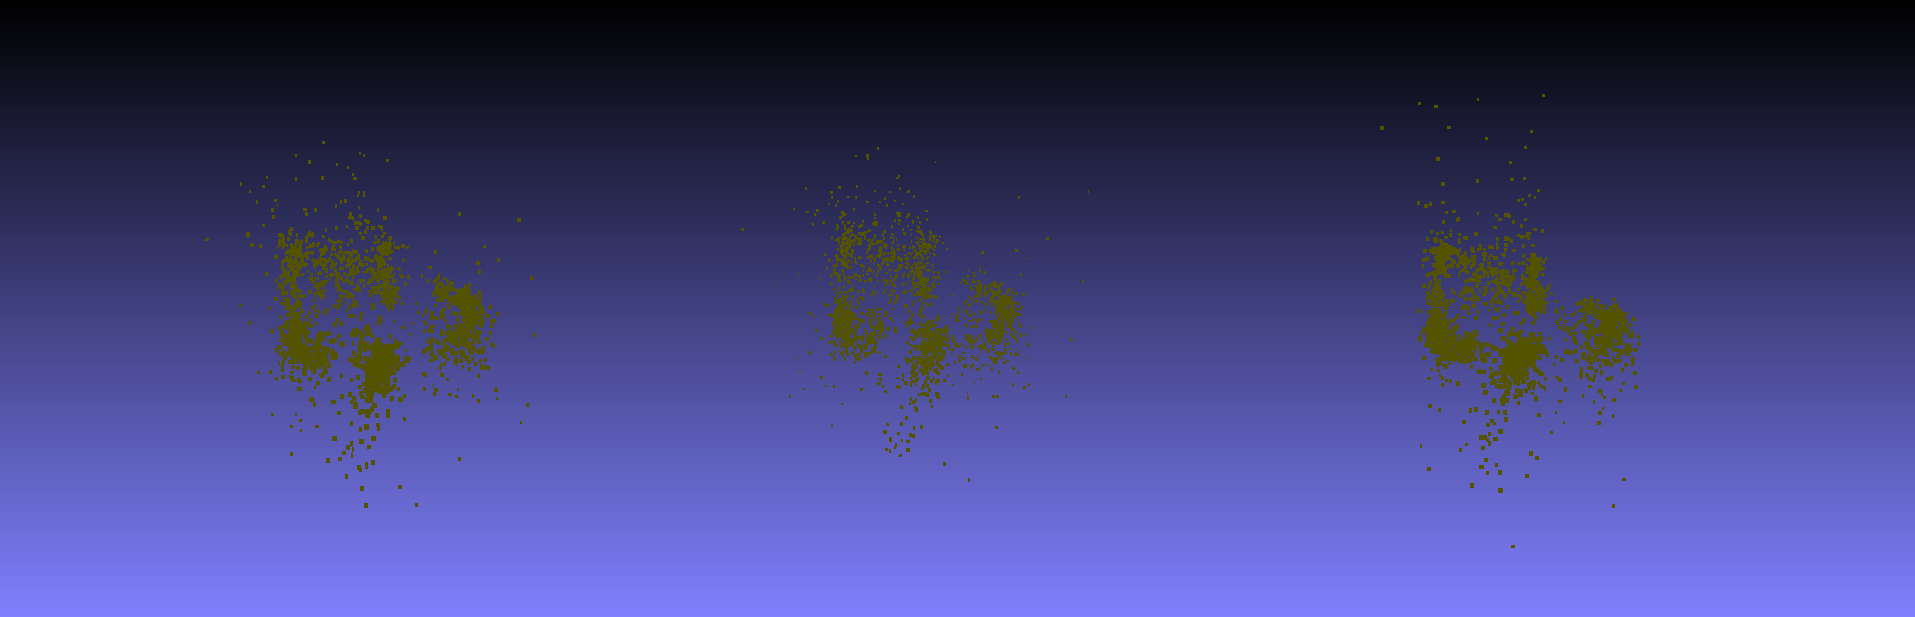
\includegraphics[width=1.0\textwidth]{raw_gan_result_400_result.png}
	\caption{Trainingsbeispiele des RAW-GAN mit den 422 Stuhldaten}
	\label{fig:Bild60}
\end{figure}
~\\\\
Für Versuchsaufbau 1.2 Latent-GAN mit Stühlen kann der Trainingsverlauf aus Abb. \ref{fig:Bild61} entnommen werden. Der Generator Loss verbessert sich zwar über mehrere Epochen gering, der Discriminator jedoch bleibt konstant auf einen seinen Ergebnisse und lässt keine starken Verbesserung des Generators mehr zu, da er die beiden Datenverteilungen perfekt unterscheiden kann. Dies führt dazu, dass der Generator kein Feedback über die Qualität seiner generierten Daten erhält und sich nicht verbessern kann.  
\begin{figure}[htbp] 
	\centering
	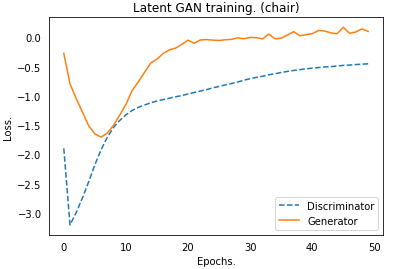
\includegraphics[width=0.5\textwidth]{latent_gan_chair_result.png}
	\caption{Trainingsverlauf des RAW-GAN mit den 422 Stuhldaten}
	\label{fig:Bild61}
\end{figure}
Beispieldatensätze, welche vom Generator nach Beendigung des Trainings erzeugt wurden in dem der latente-Code von Generator in den Decoder als Input gegeben wurde sind in Abb. \ref{fig:Bild62} zu entnehmen. Diese sind qualitativ hochwertige Daten welche eine Ähnlichkeit mit denen aus dem Trainingsdatensatz widerspiegeln. Die Ergebnisse decken sich mit den von \cite{3dgan} festgestellten Ergebnissen, in welchen das Latent-GAN qualitativ gute Stuhldaten erzeugen konnte. 
\begin{figure}[htbp] 
	\centering
	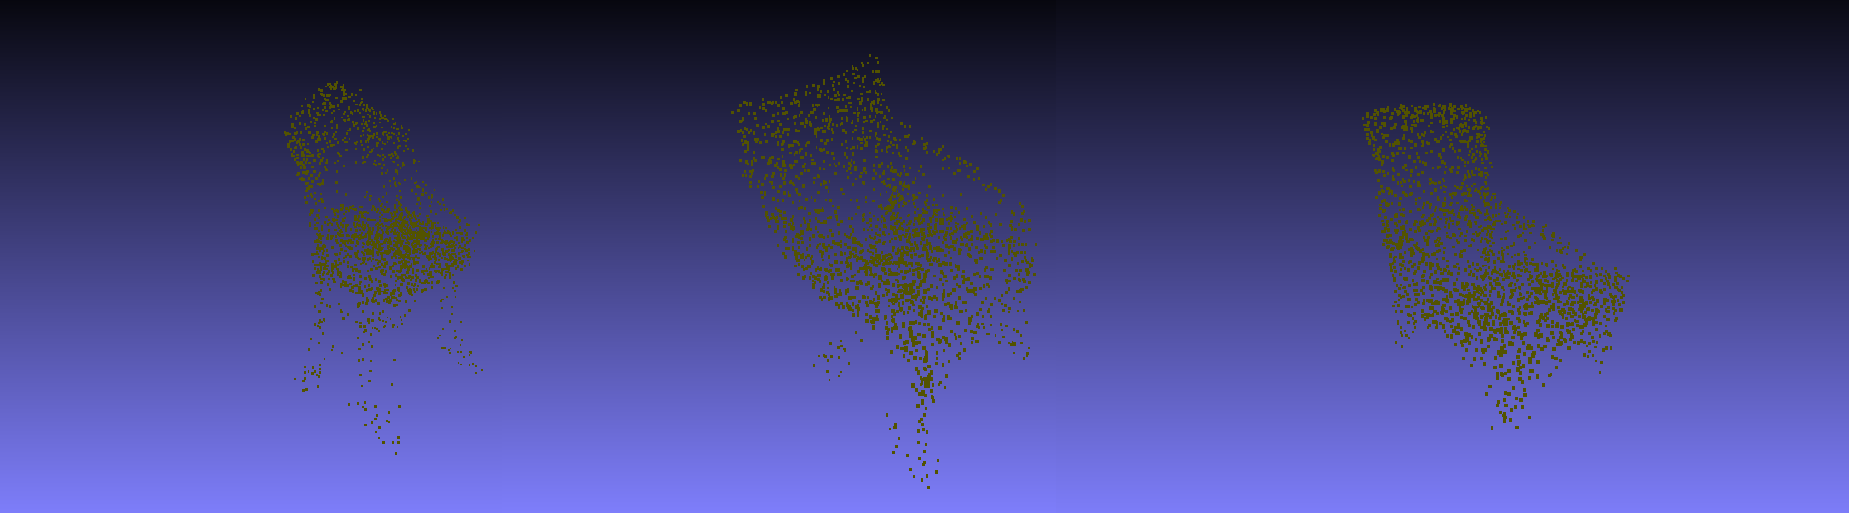
\includegraphics[width=1.0\textwidth]{latent_gan_chair_example.png}
	\caption{Trainingsbeispiele des RAW-GAN mit den 422 Stuhldaten}
	\label{fig:Bild62}
\end{figure}
~\\\\
Das Latent-GAN welches mit den Blattdaten trainiert wurde, können exemplarisch generierte Daten aus der Abb. \ref{fig:Bild64} entnommen werden. Diese zeigen eine qualitative Grundfläche, welche in der Trainingsdatengesamtheit enthalten ist. Jedoch ist festzustellen, dass es starke Punkthäufungen an gewissen Bereichen je Blatt gibt, diese sind beispielsweise im zweiten Blatt von Rechts, auf Abb. \ref{fig:Bild64} zu erkennen und mit einem roten Kreis markiert. Der Trainingsverlauf in Abb. \ref{fig:Bild63} zeigt, dass keine starken Veränderungen im weiteren Trainingsverlauf zu erwarten ist und das Training schon über mehrere Epochen stagniert.
\begin{figure}[htbp] 
	\centering
	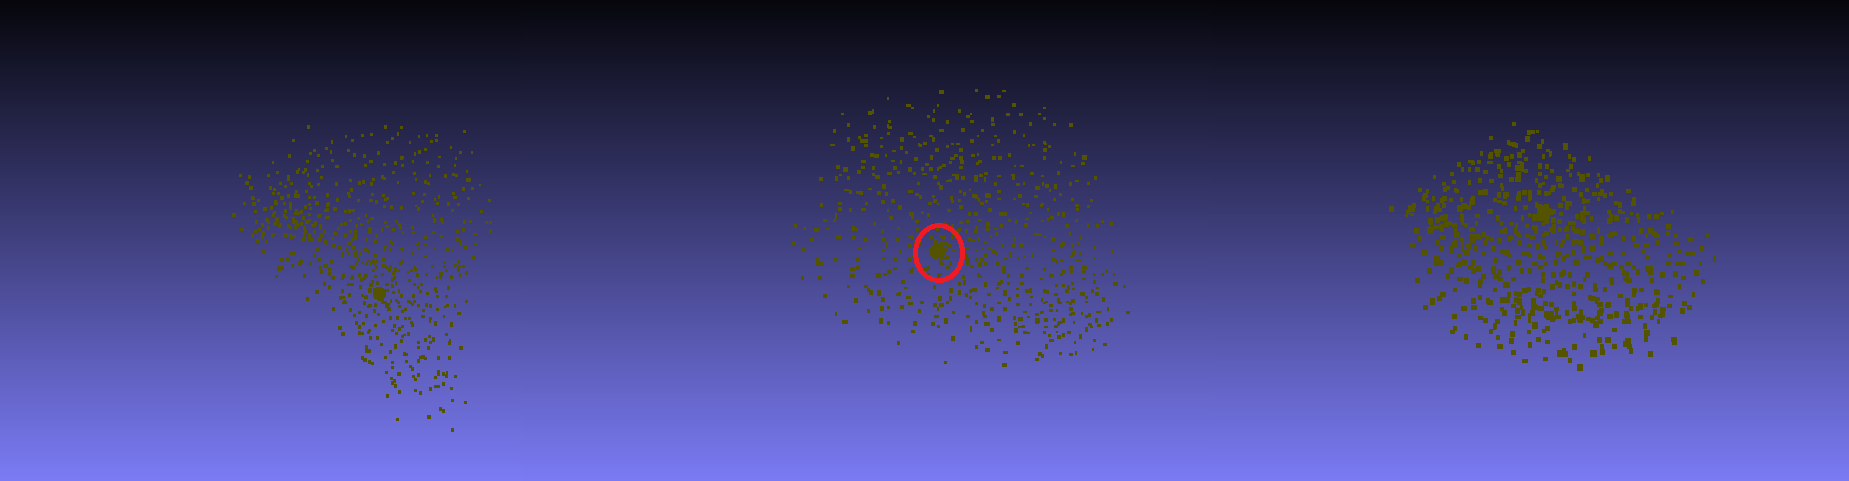
\includegraphics[width=1.0\textwidth]{latent_gan_leaf_example.png}.
	\caption{Trainingsergebnisse des Latent-GAN mit den Blattdaten}
	\label{fig:Bild64}
\end{figure}
\begin{figure}[htbp] 
	\centering
	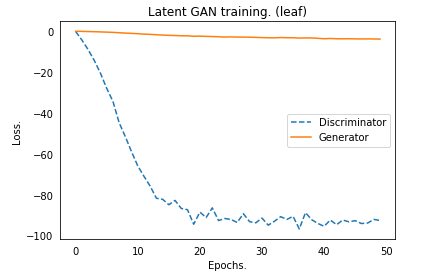
\includegraphics[width=0.6\textwidth]{Latent_gan_training_result.png}
	\caption{Trainingsverlauf des Latent-GAN mit den Blattdaten}
	\label{fig:Bild63}
\end{figure}
\pagebreak\linebreak 
Um die Ergebnisse von Testaufbau 1.2 Latent-GAN mit Stuhldaten besser vergleichbar zu machen und um ersichtlich zu machen, ob eine Erhöhung der Anzahl der Tabakblätter Daten zu einem besseren Ergebnis führen  und die Punktanhäufung sich reproduzieren lässt, wurden 422 Stuhldaten genommen um das Latent-GAN zu trainieren. In Abb. \ref{fig:Bild66} sind die exemplarisch erzeugten Daten des Generator zu entnehmen. Zu erkennen ist ein ähnlich Phonemen wie bei den Blattdaten. Hohe Punktanhäufungen finden sich an Kanten der Sitzfläche, zum Übergang der Stuhlbeine. Dadurch lassen sich Rückschlüsse darauf ziehen, dass eine Erhöhung der Daten zu einer besseren Qualität de kann. Der Trainingsverlauf kann aus Abb. \ref{fig:Bild65} entnommen werden auch dieser zeigt eine Stagnation des Verlaufs schon über mehre Epochen an und verspricht keine Erhöhung der Qualität beim weiteren Verlauf des Trainings.
\begin{figure}[htbp] 
	\centering
	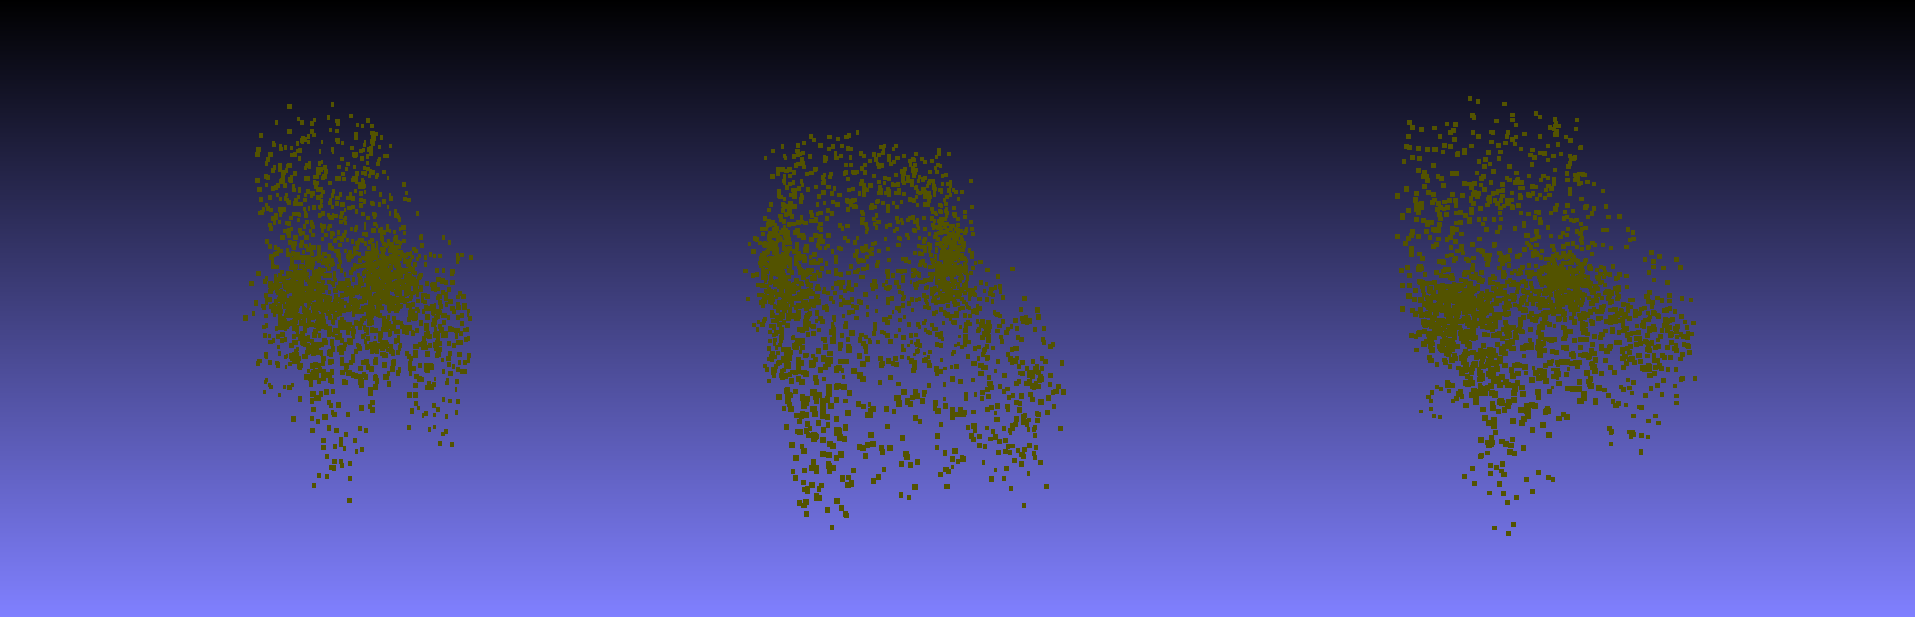
\includegraphics[width=1.0\textwidth]{raw_gan_latent_gan_chair_example_400.png}
	\caption{Traingsergebnisse des Latent-GAN mit den Stuhldaten und 400 Trainingsdaten}
	\label{fig:Bild66}
\end{figure}
\begin{figure}[htbp] 
	\centering
	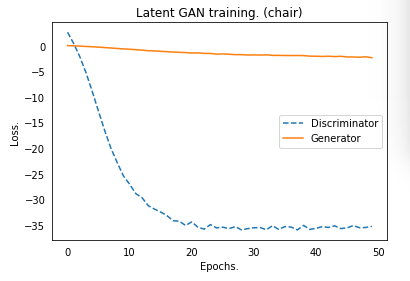
\includegraphics[width=0.6\textwidth]{raw_gan_latent_gan_chair_result_400_example.png}
	\caption{Trainingsverlauf des Latent-GAN mit den Stuhldaten und 400 Trainingsdaten}
	\label{fig:Bild65}
\end{figure}
\pagebreak\linebreak
Zusammengefasst, primär in Hinblick auf den Blattdatensatz, lässt sich feststellen, dass bei den Stuhldatensatz die Ergebnisse von Achlioptas, Panos und Diamanti\cite{3dgan} reproduziert werden konnte. Bei einen Datensatz, welcher durch Scanverfahren in diesem Beispiel Tabakblättern von realen Objekten durchgeführt wurde konnte gezeigt werden, dass durch das Latent-GAN eine erste Annäherung an qualitativ hochwertig generierten Daten zu sehen ist. Durch eine Erhöhung der Trainingsdaten lässt sich auch eine Steigerung der Qualität feststellen, wie bei den Stuhldaten durch RAW-GAN und Latent-GAN gezeigt wurde. Des Weiteren können aber keine Aussagen darüber getroffen werden, in welchem Umfang eine Qualitätssteigerung statt finden kann. 
\\\\
Die Datensätze unterscheiden sich in ihrer Aufbereitung. Die Stuhldaten sind besser auf einen Koordinatenursprung geeicht wie in Abb. \ref{fig:Bild85} festzustellen ist. Auf dieser Abbildung sind mehre Stühle zum Vergleich in ein Koordinaten System geladen. Zum Vergleich die das gleiche Konzept für die Blattdaten in Abb. \ref{fig:Bild1001}.
Zu Erkennen ist eine viel höhere Überschneidung der einzelnen Punktwolken aufeinander als bei den Blättern. Es sind dadurch gefestigter Strukturen bei den Stühlen vorhanden und dadurch weniger Varianz bei den Punktwolken untereinander. Dies hilft den Suchraum für die GANS einzuschränken und erleichtert das Training bei den Stuhldatensatz. Es müssten bessere Datenvorverarbeitungsschritte bei den Blattdaten erhoben werden, wie Beispielsweiße ein besseres festhalten des Massenzentrums aller Blätter auf den Koordinatenursprung.
\\\\ 
Außerdem sind die 6778 Stuhldaten zum Vergleich zu den 422 Blattdaten sehr gering und verschlechtern die Möglichkeit des Latenten-GAN und RAW-GAN die Grundgesamtheit der Daten abzudecken. Aus technischer Sicht könnten andere Layer Strukturen für bessere Ergebnisse sorgen. Die Bearbeitung mit Convolutio-nen-Layern auf Bilddaten hat erst den  Durchbruch bei der Rekonstruktion bei Bilddaten möglich gemacht\cite{imagerecon}. Da nun unser Generator nur aus Fully-Connected-Layern besteht, und 3D-Punktwolken komplexer sind als Bilder kann an dieser Stelle noch nachgearbeitet werden. Beispielsweise könnte ein 1D-Deconvolutional-Layer implementiert werden, welche bei Tensorflow 1.12 als Prototyp zur Verfügung steht. Eine andere Möglichkeit wäre auf die Arbeit von Cai, Zhongang  und Yu \cite{3d-conv} zurückzugreifen. Diese postuliert eine Methode für 3D-Convolution Methode, welche auf 3D-Punktwolken arbeitet und eine Invarianz im Euklidischen Raum lernt, mit deren Hilfe das Erlernen von Rotationen der Punktwolken möglich gemacht werden soll.
\begin{figure}[htbp] 
	\centering
	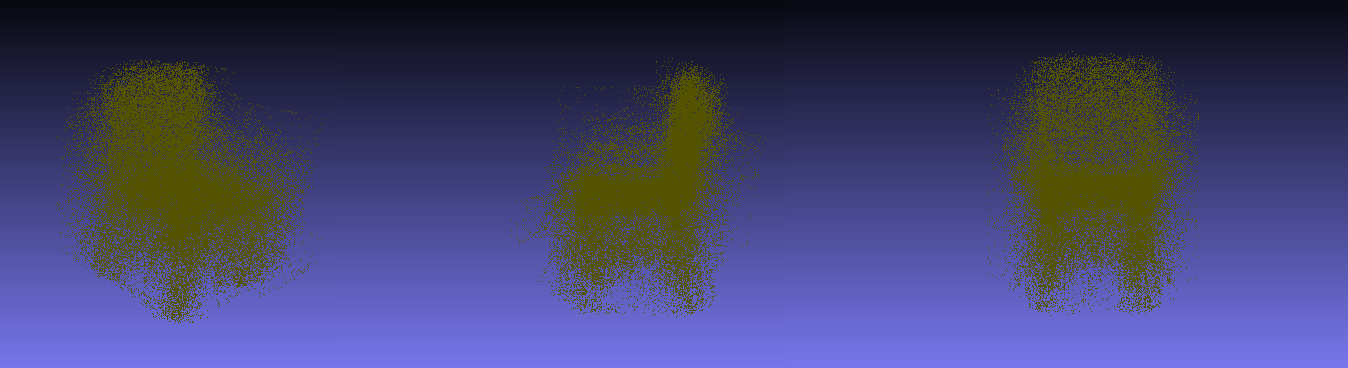
\includegraphics[width=1.0\textwidth]{chair_all.png}
	\caption{24 Stuhldaten in einen Koordinatensystem geladen}
	\label{fig:Bild85}
\end{figure}
\newpage
\subsection{Ergebnisse - Versuchsaufbau 2}
Für Versuchsaufbau 2.1, vgl. \ref{sec:versuch2-aufbau}, wurde zunächst der Autoencoder mit den zerstörten Blattdaten auf 500 Epochen trainiert, um eine komprimierte Version auf 128-D zu erlernen. Dabei wurde zunächst die in Kapitel \ref{sec:autoencoder} vorgestellte Chamfer Distanz als Distanzmaß heran genommen. Beispiel Trainingsdatensätze können Abb. \ref{fig:Bild1003} entnommen werden, mit dem jeweils erzeugten Output des Decoders in Abb. \ref{fig:Bild68}. 
\begin{figure}[htbp] 
	\centering
	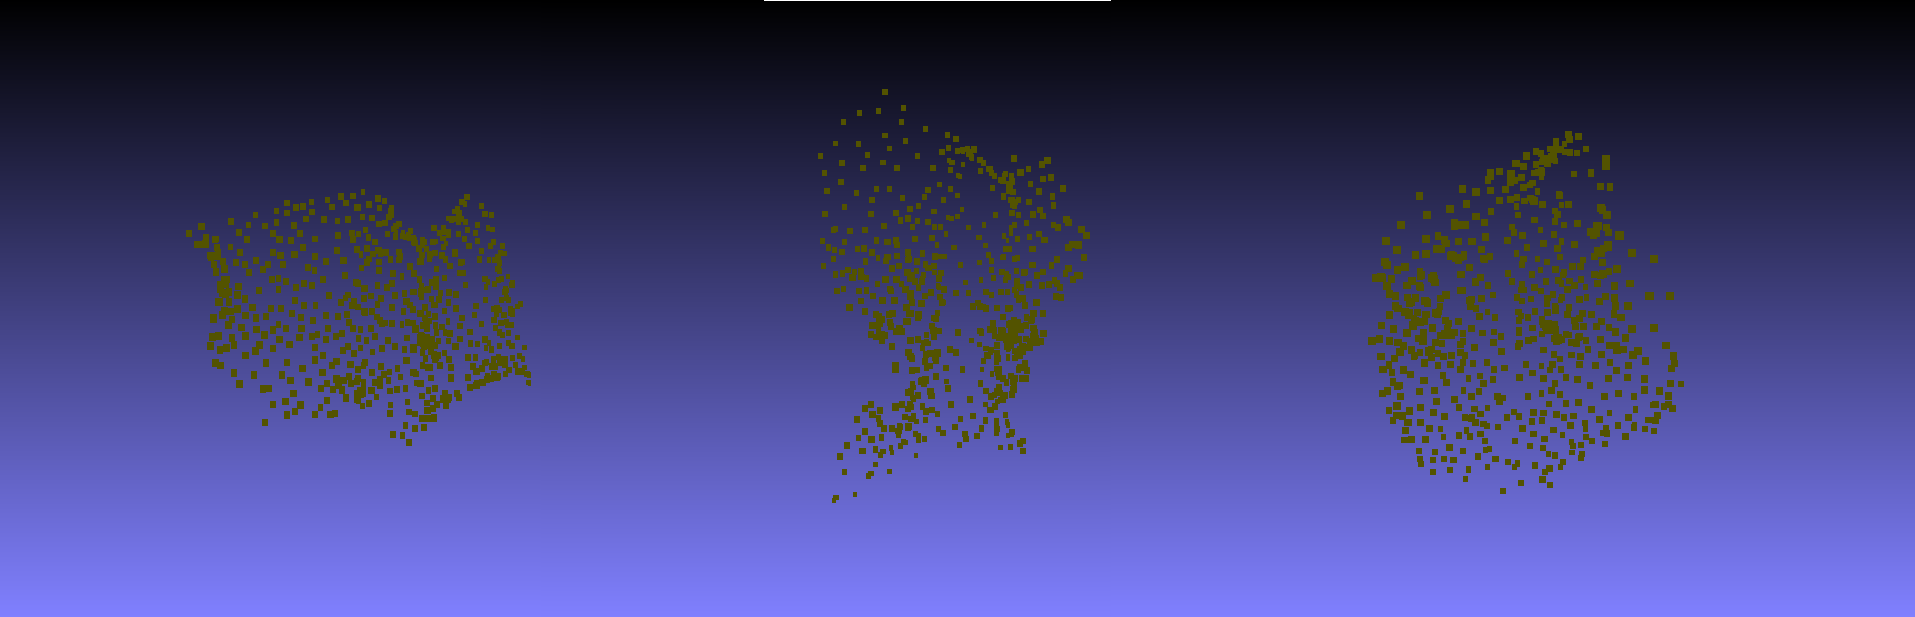
\includegraphics[width=1.0\textwidth]{autoencoder_destroyed_example_chamfer_fake.png}
	\caption{Trainingsbeispiele des Autoencoder mit CD für zerstörte Blattdaten - Output}
	\label{fig:Bild68}
\end{figure}
\begin{figure}[htbp] 
	\centering
	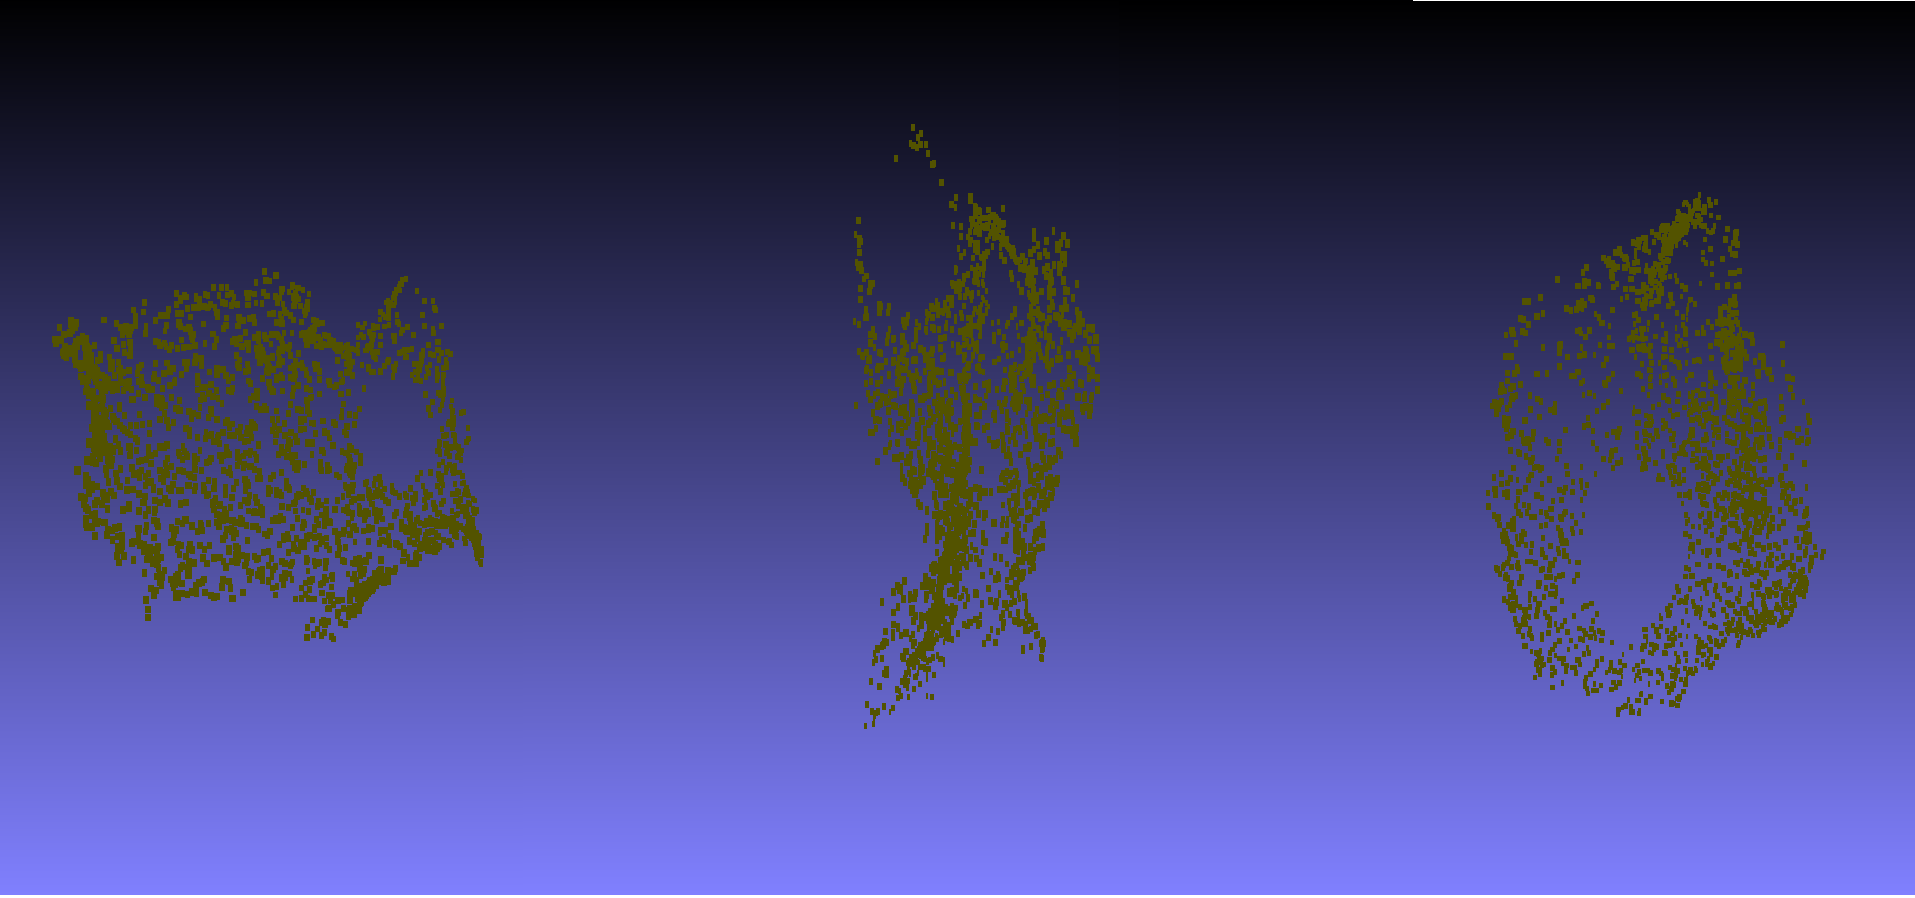
\includegraphics[width=1.0\textwidth]{autoencoder_destroyed_example_chamfer_real.png}
	\caption{Trainingsbeispiele des Autoencoder mit CD für zerstörte Blattdaten - Input}
	\label{fig:Bild1003}
\end{figure}
Wie zu erkennen ist, vervollständigt der Autoencoder mit der CD die Blätter selbstständig, obwohl das nicht als Ziel in diesem Bearbeitungsschritt vorgeben war.Es ist zu erkennen, dass die Dichte, in welcher die Punkte beim Output auf der Höhe der Löcher angeordnet sind stark von den üblichen Bereichen auf dem Blatt abweicht. 
Auch lässt der Trainingsverlauf in Abb. \ref{fig:Bild67} darauf schließend, dass der Autoencoder selbst beim weiteren Training keine bessere Codierung erlernen wird, welche die Löcher in den Blättern erzeugt, da das Training  seit Epoche 300 stagniert. Außerdem lässt der durch die CD berechnete Abstand zwischen den beiden Punktwolken keine starke Verbesserung mehr zu, da die durchschnittliche Diskrepanz nach dieser Metrik zwischen den Input x und den von Decoder erzeugten Output x` nur noch im 0.0005 Bereich liegt, wie in Abb.\ref{fig:Bild67} nach Epoche 500 abzulesen ist. Da keine verwendbaren Trainingsdaten für den Latenten C-GAN Versuchsaufbau 2.1 generiert werden konnten, soll an dieser Stelle der Versuchsaufbau 2.1 Latent C-GAN  mit Chamfer Distanz nicht weiter geführt werden. 
\begin{figure}[htbp] 
	\centering
	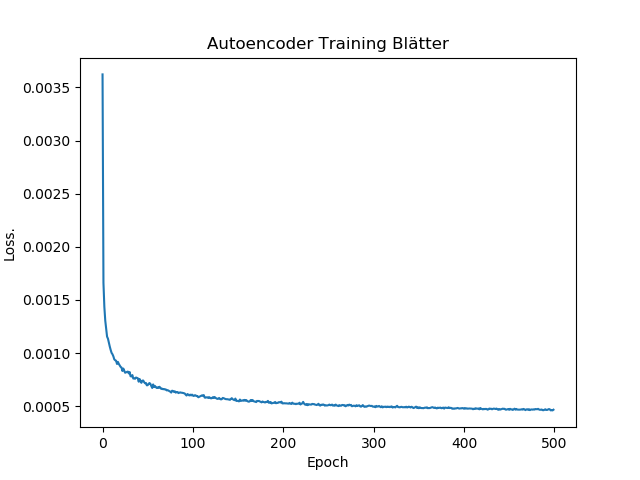
\includegraphics[width=0.6\textwidth]{autoencoder_training_blaetter_result.png}
	\caption{Trainingsverlauf des Autoencoder mit CD für zerstörte Blattdaten}
	\label{fig:Bild67}
\end{figure}
\pagebreak\linebreak 
Um ein besseres Validierungsergebnisse zu erhalten wurde Versuchaufbau 2.1 Latent-CGAN noch mit EMD Zielfunktion für Autoencoder getestet. Es wurden 800 Epochen trainiert. Die Ergebnisse sind ähnlich zu deren mit der CD vgl.\ref{sec:autoencoder}. Beispiel Trainingsinput Trainingsdatensätze können in Abb. \ref{fig:Bild71} entnommen werden mit den jeweiligen erzeugten Output des Decoders in Abb. \ref{fig:Bild72} entnommen. Wie zu erkennen ist, vervollständigt der Autoencoder mit der EMD die Blattflächen selbstständig, obwohl dies nicht als Ziel des Autoencoder ist, sondern lediglich das Erlernen einer Kodierung. Im Vergleich dazu sind die Blätter aber an der Stelle des Loches gleichmäßiger Verteilt und es gibt keine höheren Punktansammmlungen auf der Blattfläche. Wenn man die Ergebnisse mit der Hinsicht der Zielfunktion berücksichtigt liefert die CD ein besseres Ergebnis. Die Begründung hierbei ist das auf der Blattoberfläche der Blätter die Punkte gleichmässiger verteilt sind. Möchte man nun die beiden Ergebnisse ebenfalls die Qualität des Rekonstruieren messen, obwohl dies nicht das eigentliche Ziel ist, sticht die EMD hervor, da im Bereich der Löcher die Punkte gleichmäßiger verteilt sind.
\begin{figure}[htbp] 
	\centering
	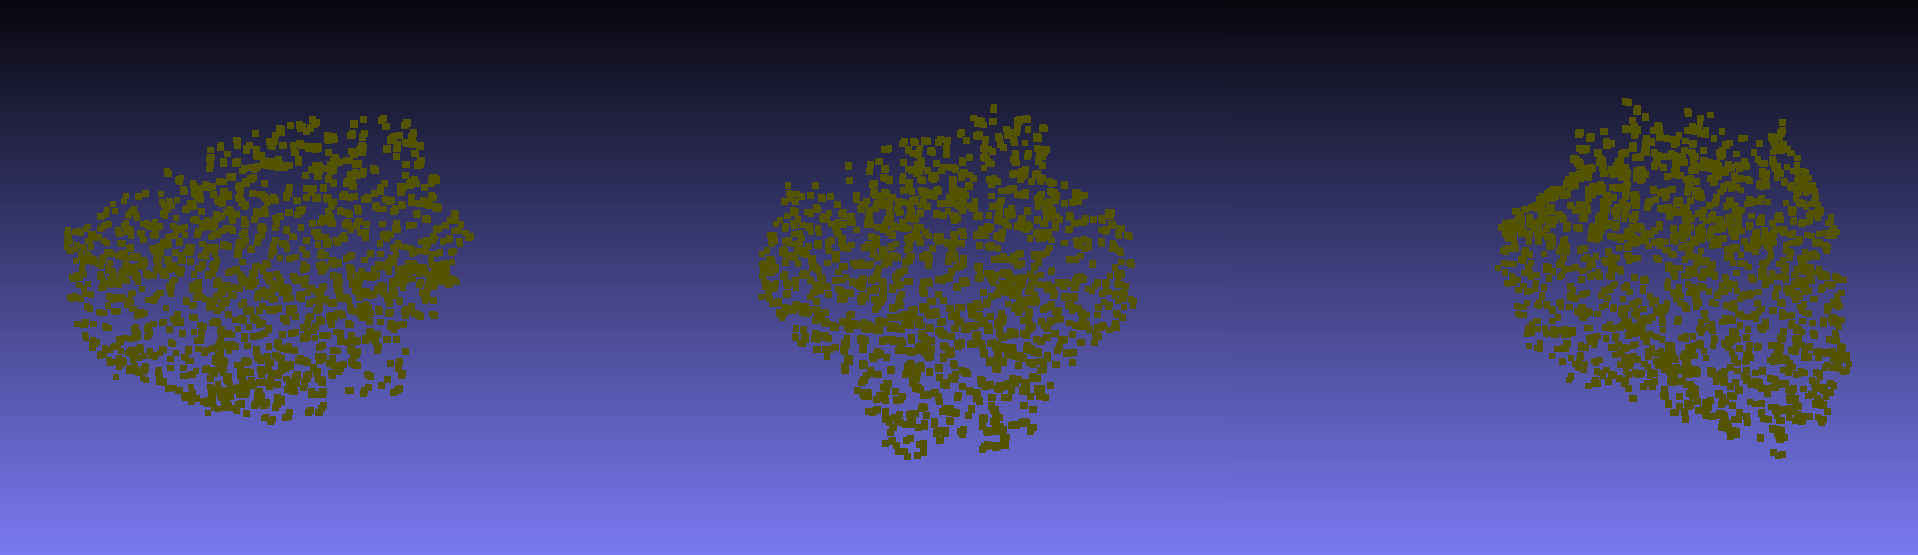
\includegraphics[width=1.0\textwidth]{repairded_emd.png}
	\caption{Trainingsbeispiele des Autoencoder mit EMD für zerstörte Blattdaten - Output}
	\label{fig:Bild72}
\end{figure}
\begin{figure}[htbp] 
	\centering
	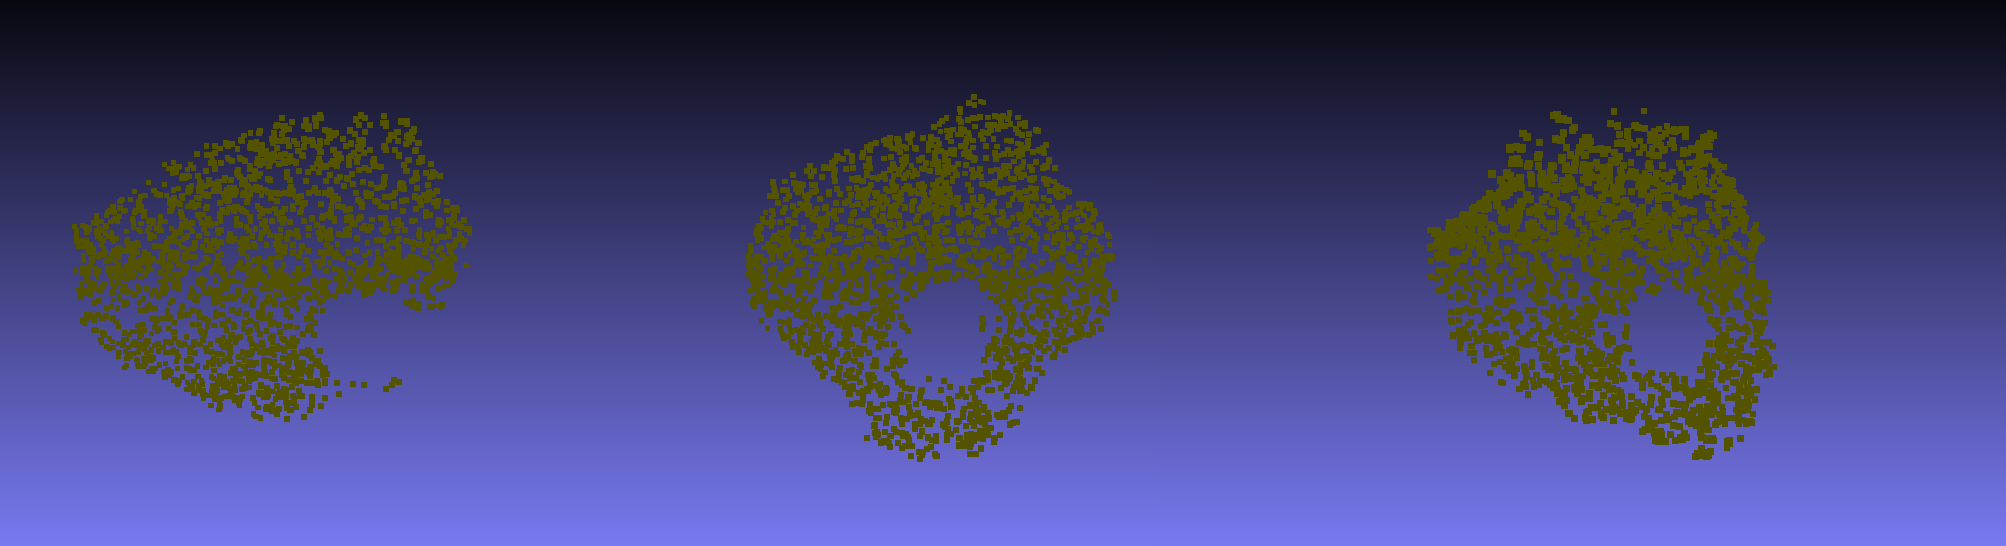
\includegraphics[width=1.0\textwidth]{input_emd.png}
	\caption{Trainingsbeispiele des Autoencoder mit EMD für zerstörte Blattdaten - Input}
	\label{fig:Bild69}
\end{figure}
\\\\
Insgesamt sind die Distanzen niedriger und die Dichte an den Löchern nimmt ab. Jedoch liefert die EMD dem positiven Nebeneffekt, dass die Blätter realistischer rekonstruiert werden. Da seit Epoche 300 das Training stagniert ist darauf zu schließend das selbst beim weiteren Training nicht die Löcher, welche in den Blättern enstehen soll, herzustellen sind. Außerdem lässt das durch die Chamfer Distanz berechnete Abstand zwischen den beiden Punktwolken keine starke Verbesserung mehr zu da die durchschnittliche Diskrepanz zwischen den Input x und den von Decoder erzeugten Output x` nur noch im 0.03 Bereich liegt wie auf Abb.\ref{fig:Bild67} in Epoche 500 abzulesen ist. Das Training entwickelt sich jedoch seit mehren Epochen nicht mehr und stagniert. Auch mit dieser Anwendung kann das Latente C-GAN nicht weitergeführt werden, da keine erfolgreichen Trainingsdaten erzeugt werden konnten.
\begin{figure}[htbp] 
	\centering
	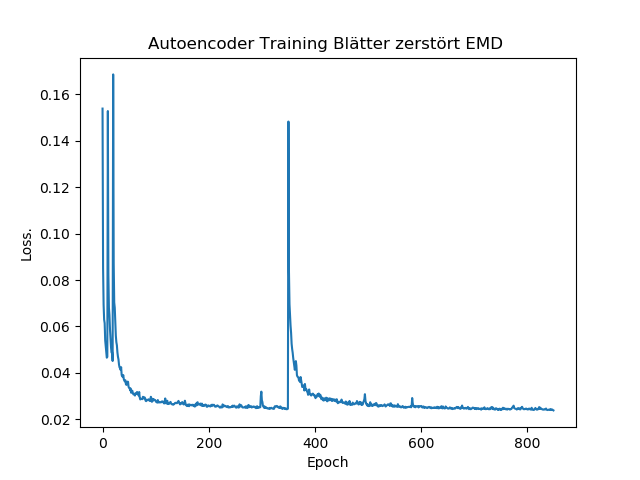
\includegraphics[width=0.7\textwidth]{autoencoder_training_bleatter_zer_result_emd.png}
	\caption{Trainingsverlauf des Autoencoder mit EMD für zerstörte Blattdaten }
	\label{fig:Bild71}
\end{figure}
\newpage
~\\\\
Für den Versuchsaufbau 2.2 RAW-CGAN mit Fully-Connected-Layern mit EMD ist auf Abb. \ref{fig:Bild75} rechts der Loss des Discriminators abgebildet und links der Loss des Generators. Der Loss des Generator sinkt zwar aber die generierten Trainingsbeispiele in Abb. \ref{fig:Bild77} ähneln keine reparierten Blätter. Der dazugehörige Input ist in Abb.\ref{fig:Bild76} zu sehen. Da der Generator schon an sein Limit gerät und keine erhebliche Verbesserung mehr möglich ist, ist festzustellen, dass durch einen Generator mit Fully-Connected-Layern keine Blattdatenrekonstruktion stattfinden kann. 
\begin{figure}[htbp] 
	\centering
	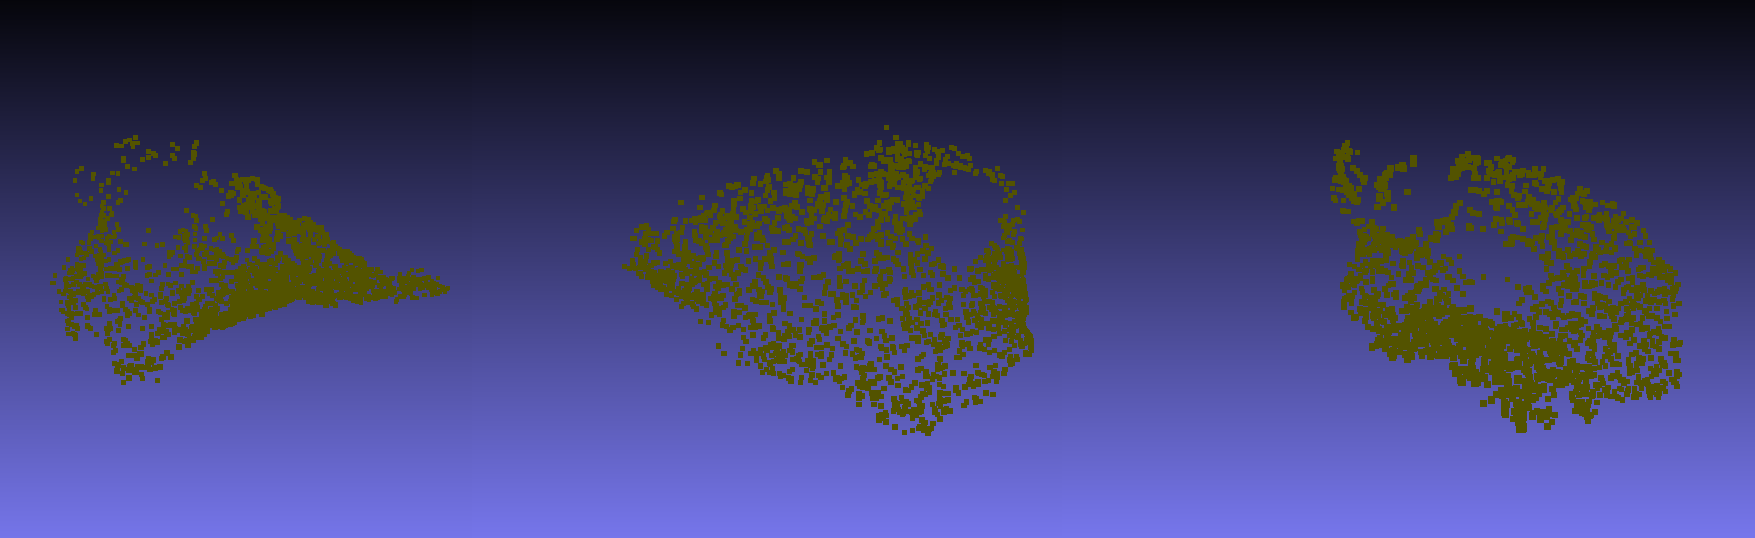
\includegraphics[width=1.0\textwidth]{reaf_fully_connected_wgan_.png}
	\caption{Der Input aus welchen vom RAW-CGAN mit EMD die Daten rekonstruiert wurden}
	\label{fig:Bild76}
\end{figure}
\begin{figure}[htbp] 
	\centering
	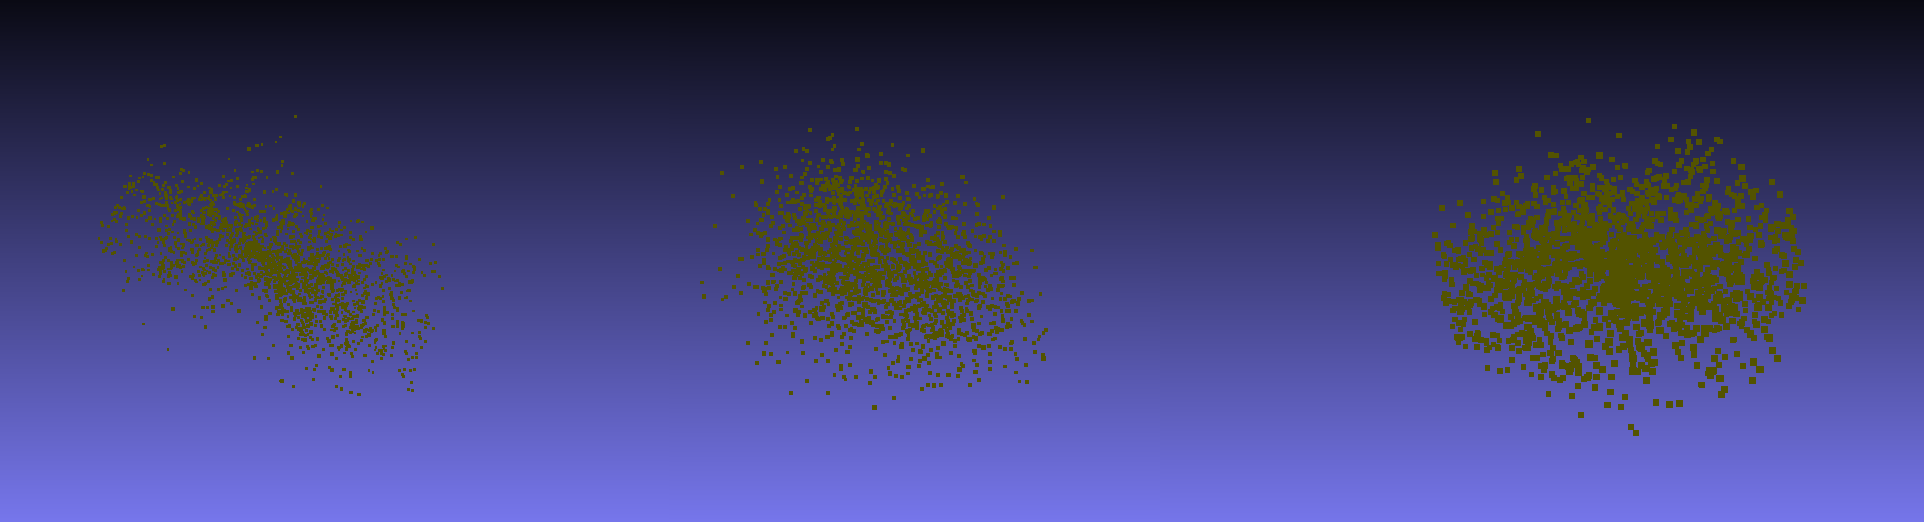
\includegraphics[width=1.0\textwidth]{fake_wgan_fully_rawcgan.png}
	\caption{Output des Generators vom RAW-CGAN mit EMD}
	\label{fig:Bild77}
\end{figure}
\begin{figure}[htbp] 
	\centering
	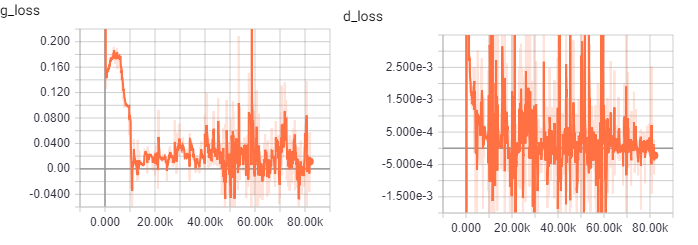
\includegraphics[width=0.8\textwidth]{wasserstein_fully_connected_rawcgan_loss.png}
	\caption{Generator und Discriminator Loss des RAW-CGAN mit EMD}
	\label{fig:Bild75}
\end{figure}
\newpage
~\\\\
In Folgenden die Ergebnisse von Testaufbau 2.2 RAW-CGAN mit Convolutional Layer im Discriminator und der Vanilla-GAN-Loss vorgestellt. Der Trainingsverlauf vom Generator und Discriminator kann Abb. \ref{fig:Bild79} entnommen werden. Die Sprünge sehen auf den ersten Blick sehr stark, aus beachtet man aber die Scalenwerte auf der Y-Achse des Generators, bewegt sich der Loss zwischen 0.691 und 0,696. Dies lässt auf keine starke Verbesserung schließen. Der Discriminator kann die Unterscheidung von Fake und Real Datensatz perfekt erkennen. Das Training läuft über mehre Epoche konstant hinweg und lässt auch für einen längeren Durchlauf auf keine Verbesserung schließen. Einige Beispieltabakblätter welche vom Generator erstellt wurden sind können aus Abb. \ref{fig:Bild80} zu entnehmen so wie der dazu gehörige Input aus Abb. \ref{fig:Bild78}. Diese sind jedoch keine hohe Ähnlichkeit zu Blätter zu erkennen, man erkennt eine Verbesserung zum RAW-CGAN mit Fully-Connected-Layern, da sich bessere Blattränder abbilden jedoch führen starke Punktansammlungen zu keinen dichten Blattflächen. Da es nach der Loss Funktion keine gravierenden Veränderungen mehr zu erwarten sind, kann festgehalten werden das keine Rekonstruktion von zerstörten Blattdaten mit den in Kapitel \ref{sec:versuch2-aufbau} beschriebenen RAW-CGAN mit Convolutional-Layer und Vanilla-GAN-Loss, möglich ist.
\begin{figure}[htbp] 
	\centering
	\includegraphics[width=1.0\textwidth]{dcpgan_ws_fake.png}
	\caption{Der Output aus welchen vom RAW-CGAN mit Convolutional Layern die Daten rekonstruiert wurde}
	\label{fig:Bild80}
\end{figure}
\begin{figure}[htbp] 
	\centering
	\includegraphics[width=1.0\textwidth]{dc_pgan_ws_real.png}
	\caption{Der Input aus welchen vom RAW-CGAN mit Convolutional Layern die Daten rekonstruiert wurden}
	\label{fig:Bild78}
\end{figure}
\begin{figure}[htbp] 
	\centering
	\includegraphics[width=1.0\textwidth]{cgan_loss_vanilla.png}
	\caption{RAW-CGAN mit Convolutional-Layern und Vanilla-GAN-Loss}
	\label{fig:Bild79}
\end{figure}
\newpage
~\\\\
Zuletzt erfolgen die Ergebnisse von Testaufbau 2.2 RAW-CGAN mit Deconvo-lutional-Layer mit der Wasserstein-Metric, was mit den nicht komprimierten Daten trainiert wird.  Der Trainingsverlauf vom Generator und Discriminator kann Abb. \ref{fig:Bild1001} entnommen werden.  Der Verlauf des Discriminator Loss arbeitet sich konstant nach unten und hat zwei Ausbrecher welche aber kein Einfluss auf den weiteren Trainingsverlauf hat, da der Generator durch den Gradienten kein Aufschwung erlangt. Der Generator springt zwar noch am Ende des Trainings aber die Sprünge sind in einen so niedrigen Intervall das keine große Veränderung mehr erwartet werden kann. Die vom Generator generierten Outputs in Abb. \ref{fig:Bild82}, und deren dazugehöriger Input in Abb. \ref{fig:Bild83} zeigen bereits die Umrisse der Blätter auf jedoch sind die Blattflächen nicht gebildet. 
\begin{figure}[htbp] 
	\centering
	\includegraphics[width=1.0\textwidth]{cgan_ws_loss.png}
	\caption{Discriminator und Generator Loss RAW-DGAN mit Convolutional-Layer und Wasserstein Metrik}
	\label{fig:Bild1001}
\end{figure}
\begin{figure}[htbp] 
	\centering
	\includegraphics[width=1.0\textwidth]{raw_cgan_ws_fake.png}
	\caption{Der Output aus welchen vom RAW-CGAN mit Convolutional Layern die Daten rekonstruiert wurde}
	\label{fig:Bild82}
\end{figure}
\begin{figure}[htbp] 
	\centering
	\includegraphics[width=1.0\textwidth]{raw_cgan_ws_real.png}
	\caption{Der Input aus welchen vom RAW-CGAN mit Convolutional Layern die Daten rekonstruiert wurden}
	\label{fig:Bild83}
\end{figure}
Fast man Versuchsaufbau 2 zusammen ist festzustellen das in Versuchsaufbau 2.1 abgebrochen werden musste da die Autoencoder nicht fähig waren, die zerstörten Trainingsdaten zu erlernen. Jedoch konnten sie die Daten rekonstruieren, obwohl dies nicht als Ziel für die Autoencoder definiert war. Ob eine praktische Anwendung hier durch ermöglicht ist und ob diese Rekonstruktion nur für die Form von Blätter möglich ist, oder Beispielsweise auch ähnliche Ergebnisse beim Stuhldaten Satz liefert, muss in folge Arbeiten geprüft werden.
\\\\
Die beiden Zielfunktionen des Autoencoder, CD und EMD, hatten beide ein ähnliches Problem zu erkennen, welcher Punkt in Punktwolke x der dazugehörige Punkt in Punktwolke y ist, auf welchen die Optimierung statt finden soll. Beide lösten dies indem sie die nähsten Nachbarn eines Punktes aus der anderen Punktwolke suchen.  Jedoch kann dieses Mapping zu Problemen führen, wie man in Abb.\ref{fig:Bild1005} erkennen kann. Die rote Punktwolke ist der erste Versuch des Autoencoders die grüne Punktwolke zu kopieren. Eine Zuordnung in diesem Stadium, welcher Punkt in Rot zu Grün gehört ist sehr schwierig. Dadurch resultiert das Punkte in Zentrum eher als nächster Nachbar identifiziert werden. Im weiteren Trainingsverlauf dehnt die rote Punktwolke sich aus, lässt aber durch die Ansammlung im Zentrum und der bijektive Zuordnung der Punkte zueinander, nicht zu das sich die Löcher bilden. Für eine weitere Nutzung könnte an dieser Stelle angesetzt werden und andere Zielfunktionen für Autoencoder mit Punktwolken entwickelt werden. Oder den Encoder dahingehend umbauen das der Output frühere Lernepochen eher der Grundform eines Blattes ähnelt. 
\begin{figure}[htbp] 
	\centering
	\includegraphics[width=1.0\textwidth]{problem_autoencoder.png}
	\caption{Rot der Output des Autoencoders in Epoche 1, Grün der Input des Autoencoders }
	\label{fig:Bild1005}
\end{figure}
Im Versuchsaufbau 2.2 zeigen sich mit der Verwendung von Convolutional-Layer im Discriminator bessere Ergebnisse. Ein qualitativer Unterschied zwischen dem Versuchsaufbau 2.2 RAW-CGAN mit Convolutional-Layer und Vanilla-GAN oder Wasserstein Metrik lässt sich nicht feststellen. Jedoch lässt die Convolutional-Layer das erlernen der Latenten-Struktur besser gelingen. Eine Rekonstruktion ist aber auch mit diesen Model nicht möglich. Jedoch kann nicht ausgeschlossen sein das GAN durch andere Aufbauten wie Beispielsweise mit 1D-Deconvolutional-Layer, implementiert werden, welche bei Tensorflow 1.12 als Prototyp zur Verfügung steht. Eine weitere Möglichkeit wäre auf die Arbeit von Cai, Zhongang  und Yu \cite{3d-conv} anzusetzen dieser postuliert eine Herangehensweise für 3D-Convolution Methode, welche auf 3D-Punktwolken arbeitet und eine Invarianz im Euklidischen Raum lernt mit deren Hilfe es möglich sein soll Rotationen der Punktwolke zu erlernen. Durch diese neuen Module könnte das Erlernen des latenten Raumes von 3D-Punktwolken möglich gemacht werden und das letztendliche Ziel, 3D-Punktwolken zu rekonstruieren erreicht werden. 
\newpage
\section{Zusammenfassung und Diskussion }

Verglichen mit anderen Daten, wie Bildern oder Audio, bleiben 3D-Daten eine Herausforderung, da ihr Suchraum erheblich höher ist, wie auch in Kapitel \ref{sec:3dprobleme} thematisiert. Durch den Informationsgehalt von Punktwolken erhöht sich der Suchraum für GANs und stellt Forscher vor neue Herausforderungen. Die Fragestellungen, welchen in dieser Arbeit nachgegangen werden sollte, lauten:
\begin{description}
\item[Fragestellung 1] Können durch GANs 3D-Punktwolken von Tabakblättern erlernt werden um neue Datensätze zu generieren?\\
\item[Fragestellung 2] Können durch GANs 3D-Punktwolken von Tabakblättern, die von ihrem Urzustand abgebracht wurden, rekonstruiert werden? 
\end{description}
Es konnte festgestellt werden, dass die Fragestellung 1 (vgl. \ref{sec:versuch1-aufbau}) positiv beantwortet werden kann, jedoch noch Verbesserungen in der Qualität der durch GANs generierten 3D-Punktwolken möglich sind. Der Aufbau, welcher derzeit die besten Ergebnisse hervorbringt, ist das Latent-GAN. Aber auch beim RAW-GAN für Punktwolken ist eine Erhöhung der Qualität festzustellen, wenn mehr Daten zur Verfügung stehen. Außerdem könnte eine systematischere Datenvorverarbeitung der Trainingsdaten bessere Ergebnisse hervor bringen, wie beispielsweise eine Zentrierung der Massepunkte jedes Blattes auf den Koordinaten Ursprung, oder eine einheitlichere Ausrichtung der Blattflächen zu einem Fixpunkt im Euklidischen Raum. Beim strukturellen Aufbau des GAN könnte ein 1D-Deconvolutional-Layer implementiert werden, welche bei Tensorflow 1.12 als Prototyp zur Verfügung steht. Eine andere Möglichkeit wäre es, auf die Arbeit von Cai, Zhongang  und Yu \cite{3d-conv} zurückzugreifen. Diese postuliert eine Herangehensweise für 3D-Convolution Methode, welche auf 3D-Punktwolken arbeitet und eine Invarianz im Euklidischen Raum lernt, mit deren Hilfe das Erlernen von Rotationen der Punktwolken möglich gemacht werden soll.
\\\\
Zu Fragestellung 2, welche in Kapitel \ref{sec:versuch2-aufbau} überprüft wurde, ist festzuhalten, dass der Aufbau des Latent-CGAN abgebrochen werden musste, da der Autoencoder die zerstörten Trainingsdaten nicht erlernen konnte und somit eine weitere Durchführung des Versuchsaufbaus unmöglich macht. Jedoch war festzustellen, dass die Autoencoder die Löcher in den Blättern mit Punkten füllten und somit eine Rekonstruktion möglich machten. Dies ist auf die beiden Zielfunktionen des Autoencoder zurück zuführen, welche durch das Distanzmaß zwischen 2 Punktwolken dafür sorgt, dass die Punktwolken gedehnt werden. Ob dadurch eine praktische Anwendung möglich ist und ob diese Rekonstruktion nur für die Form von Blättern gilt, oder beispielsweise auch ähnliche Ergebnisse beim Stuhl Datensatz möglich sind, muss in zukünftigen Arbeiten geprüft werden. Dies kann durch die gleiche Datenverarbeitung mit den Sphären für Stuhldaten überprüft werden. 
\\\\
Das RAW-CGAN zeigte bessere Ergebnisse mit der Verwendung von Convolutional-Layern im Discriminator. Jedoch war auch mit diesem Versuchsaufbau die Rekonstruktion von Daten nicht möglich. Es zeigte sich doch eine Verbesserung mit den Convolutional-Layern, im Vergleich zu den Fully-Connected Layern. Da es bei der Rekonstruktion von Bildern erst durch den Einsatz verbesserter Convolution Methoden ermöglicht wurde Bilder zu rekonstruieren und zu verändern \cite{imagerecon} und diese Convolution speziell auf 2D-Daten entwickelt wurde. Daher lässt sich nicht ausschließen, dass durch Verwendung von Layern, welche speziell für 3D-Daten entwickelt wurden, bessere Ergebnisse hervorgebracht werden können. Auch hier kann, wie bei Fragestellung 2, beispielsweise mit 1D-Deconvolutional-Layer implementiert werden. Eine andere Möglichkeit wäre es, auf die Arbeit von Cai, Zhongang  und Yu \cite{3d-conv} aufzubauen. Diese postulieren eine Herangehensweise für die 3D-Convolution Methode, welche auf 3D-Punktwolken arbeitet und eine Invarianz im Euklidischen Raum lernt, mit deren Hilfe es einfach sein soll, Rotationen der Punktwolke zu erlernen. Durch diese neuen Module könnte das Erlernen des latenten Raumes von 3d-Punktwolken möglich gemacht werden und das letztendliche Ziel, 3D-Punktwolken zu rekonstruieren, erreicht werden.  Eine weitere Möglichkeit ist es auch, die Zielfunktion von GAN zu ändern, wie in der Arbeit von Zhu, Jun-Yan und Park \cite{pix2pix}, mit ihrem Pix2Pix Model. In diesem verwenden sie die C-GAN Loss Funktion und ändern diese um zusätzlich zur üblichen Loss-Funktion auch die Differenz zwischen Generator Output und dem dazugehörigen Urzustand des Trainingsdatensatz zu berechnen und addieren dies zur Loss-Funktion. Dieses Verfahren könnte für Punktwolken übernommen werden und mit der CD oder EMD implementiert werden. Obwohl die qualitative Rekonstruktion von Punktwolken von Tabakblättern nicht zufriedenstellend erreicht werden konnte, besteht dennoch Potential, die in der vorliegenden Abhandlung thematisierten Forschungsfragen in zukünftigen Arbeiten weiter zu verfolgen.
\newpage
\listoffigures
\newpage
\bibliographystyle{apacite}
\bibliography{mybib}
\end{document}
